% vim: spelllang=fr

\documentclass[../main.tex]{subfiles}
\graphicspath{{\subfix{../Figures/Chap4/}}}
\begin{document}

\begin{itshape}
    Dans ce dernier chapitre, on établit et applique des indices de cyclogénèse, construits par régression de Poisson, non plus dans le monde de la réanalyse et
    des observations, mais dans le monde du modèle avec ARPEGE-Climat. L'ajout de nouveaux prédicteurs dans la régression est exploré, et une attention
    particulière est portée à la recherche de tendances à long terme. Les indices sont ensuite appliqués à des simulations à climat plus chaud avec ARPEGE
    utilisé dans sa configuration basculée-étirée sur les antilles et sur le bassin Sud-Indien.
\end{itshape}

\minitoc
\newpage

%--------------------------------------
\section{Introduction}

Dans le \cref{chap:chapitre_3}, nous avons construit des indices de cyclogénèse par régression de Poisson en prenant la réanalyse ERA5 comme source pour
l'environnement de grande échelle, et la base de données observationnelle IBTrACS comme référence pour les observations. Dans ce chapitre, nous nous
intéresserons à l'utilisation d'indices de cyclogénèse dans des simulations climatiques réalisées avec ARPEGE-Climat. [En cours]

Il faut justifier le fait de faire un indice de cyclogénèse sous perfusion Niño 3.4 pour essayer de donner de l'amplitude et de la corrélation à la variabilité
interannuelle. Si on demande, on le fait dans le monde du modèle parce que les travaux ERA5 sont plutôt une introduction aux outils et aux méthodes utilisées
pour les indices, notamment pour l'aspect validation de la reproduction de la méthodologie de Tippett, et la déclinaison en régression à l'échelle du bassin ;
indispensable pour Niño mais aussi pour les runs climat futur puisqu'elles sont faites en basculée-étirée.

\section{Utilisation d'un indice Niño dans une régression de Poisson}\label{sec:indice_ONI}

On s'intéresse ici à l'ajout explicite du signal du mode de variabilité ENSO (\textit{El Niño-Southern Oscillation}) dans un indice de cyclogénèse construit par
régression de Poisson. Il s'agit de voir si ce nouvel apport d'information est susceptible d'introduire de l'amplitude dans la variabilité interannuelle inférée
par un tel indice, et de voir si ce prédicteur peut, ou non, améliorer au moins localement la représentation de la variabilité interannuelle.

\subsection{Données et Méthodes}

\subsubsection{Simulation historique forcée avec ARPEGE-Climat}

Nous utilisons ici le modèle ARPEGE dans sa version 6.3 à haute résolution, dans la même configuration que dans
\textcite{chauvin_future_2020,cattiaux_projected_2020}. Cette version du modèle est quasiment identique à celle utilisée dans le modèle couplé CNRM-CM6-1
\parencite{voldoire_evaluation_2019} et CNRM-ESM2 \parencite{seferian_evaluation_2019}, participant à CMIP6 \parencite{eyring_overview_2016} et HighResMIP
\parencite{haarsma_highresmip_2020}. Une description détaillée de toutes les nouveautés dans cette version d'ARPEGE par rapport à la version précédente (5.2)
est disponible dans \textcite{voldoire_evaluation_2019}, tandis que la version précédente est décrite dans \textcite{voldoire_cnrmcm5_2013}. Nous ne précisons
alors ici que les éléments particulièrement pertinents pour la simulation des cyclones tropicaux. Ainsi, le modèle est constitué du schéma physique PCMT
(\textit{Prognostic Condensates Microphysics and Transport}), incluant le schéma convectif de \textcite{piriou_approach_2007,gueremy_continuous_2011}, offrant
une paramétrisation de la convection profonde et peu profonde. Cette version voit également l'ajout de dix nouvelles variables pronostiques\footnote{Les
variables dites \textquote{pronostiques} se distinguent des variables dites \textquote{diagnostiques} en cela que leur évolution temporelle est décrite par la
résolution d'une équation dans le modèle numérique. Par opposition, les variables diagnostiques (par exemple, l'humidité relative) sont dérivées des variables
pronostiques (température, pression, humidité spécifique...).}, en plus des six déjà présentes. Spécifiquement, ARPEGE 6.3 calcule désormais l'évolution du
contenu en eau liquide et solide, précipitée ou nuageuse, de l'énergie cinétique turbulente et de la vitesse verticale convective. La paramétrisation de la
microphysique provient du schéma de \textcite{lopez_implementation_2002}, tandis que le schéma de turbulence est issu de \textcite{cuxart_turbulence_2000}. Le
modèle possède \num{91} niveaux verticaux, jusqu'à \hPa{0.01}, et la couche de mélange atmosphérique est caractérisée par \num{15} niveaux verticaux en dessous
de \m{1500} d'altitude.

La simulation utilisée ici est une simulation historique sur la période \num{1979}~--~\num{2010} et sur une grille T359, de taille \num{720} (longitude)
$\times$ \num{360} (latitude), donc à une résolution horizontale de \ang{0.5}, soit d'environ \km{50} à l'équateur. La simulation est forcée par la SST et la concentration
en glace de mer issues d'observations et provenant de la base de données HadISST1 \parencite{rayner_global_2003}.

\subsubsection{Cylogénèses simulées}\label{sec:tracking_arpege}

Les cyclones tropicaux sont détectés à l'aide du schéma de détection du CNRM \parencite{chauvin_response_2006}, amplement décrit dans le \cref{chap:chapitre_2},
notamment dans la \cref{sec:eval_tracker_ERA5}. Le schéma de détection a été appliqué aux champs 6-horaires du modèle avec : un seuil de vorticité
\textbf{VOR}~$=$~\SI{20e-5}{\per\second} ; un seuil de vent \textbf{RES}~$=$~\ms{13}, un seuil d'anomalie de température \textbf{TANOM}~$=$~\SI{1}{\kelvin} ; un
seuil de profil vertical de température \textbf{PT}~$=$~\SI{-2}{\kelvin} ; un seuil de profil vertical de vitesse du vent \textbf{PW}~$=$~\ms{5}, et enfin un
paramètre de relaxation des trajectoires \textbf{REL} fixé à \SI{20e-5}{\per\second}. Ces paramètres se distinguent notablement de ceux utilisés pour ERA5 dans
\textcite{dulac_assessing_2023} par le seuil vorticité (respectivement \SI{15e-5}{\per\second}) et surtout par le seuil de vitesse du vent à la surface
(respectivement \ms{5}). Rappelons en effet que le modèle ARPEGE, en particulier cette version précise du modèle, est connue pour simuler des cyclones tropicaux
intenses par rapport à la résolution du modèle \parencite{roberts_impact_2020,chauvin_future_2020} (voir aussi \cref{sec:cyclones_dans_modèles} du
\cref{chap:chapitre_1}, notamment la \cref{fig:roberts_PV_resolution}, \vpageref{fig:roberts_PV_resolution}). Il convient néanmoins de préciser que
contrairement au \cref{chap:chapitre_2}, le choix des seuils de détection utilisés pour détecter les TC dans cette simulation n'ont pas fait l'objet d'une
analyse quantitative des performances ---~une telle analyse serait par ailleurs impossible étant donné qu'il n'existe pas de trajectoires de référence pour les
pures simulations atmosphériques. Avant post-traitement des trajectoires, la fréquence d'occurrence annuelle moyenne de cyclogénèses est de \num{80.7} TC par
an. À titre de référence, IBTrACS sur la même période indique \num{82.9} TC par an.

Nous appliquons en post-traitement le filtre des systèmes de moyennes latitudes basé sur le diagnostique du jet subtropical (STJ), décrit et illustré dans la
\cref{sec:filtrage_mid_latitudes} (\cref{chap:chapitre_2}). Ce filtre est choisi ici ---~en dépit des réserves exprimées dans le \cref{chap:chapitre_2}~--- en
raison de sa relative simplicité à implémenter, notamment par rapport au filtre du $V_U^T$ qui a lui été préféré dans \textcite{dulac_assessing_2023}. En effet,
l'emploi du filtre du $V_U^T$ comme post-traitement nécessite de traiter en profondeur les champs spatiaux 3D du modèle centrés sur les positions des TC
préalablement identifiés, une opération qui est à la fois techniquement complexe et chronophage. En comparaison, la détermination de la limite équatoriale du
STJ peut être faite une fois pour toutes, et n'est pas à proprement parler dépendante des trajectoires identifiées, au sens où il n'est pas nécessaire de
répéter le diagnostique pour appliquer le filtre à de nouvelles trajectoires issues de la même simulation. En outre, \textcite{bourdin_intercomparison_2022}
montrent que le filtre du STJ parvient très efficacement à filtrer les systèmes de moyennes latitudes, lorsqu'appliqué à plusieurs schémas de détection sur
ERA5. Rappelons brièvement que la latitude du STJ est déterminée en prenant la limite équatoriale des points où le module du vent à \hPa{200} (lissé sur trois
mois glissants) est supérieur à \ms{25} et où la composante zonale (lissée de la même façon) est supérieure à \ms{15}. En pratique, puisqu'on s'intéresse aux
cyclogénèses et qu'on ne garde pour cela que les premières échéances des trajectoires, le filtre consiste à retirer les points situés au delà de la latitude du
STJ.

La \cref{fig:track_density_PRE625REFT359x} présente la densité annuelle moyenne (sur \num{30} ans) des premières échéances des trajectoires détectées dans la
simulation ARPEGE ---~assimilées aux cyclogénèses~--- après application du filtre du STJ. Avec le filtre du STJ, la fréquence annuelle moyenne est réduite à
\num{60.8} TC par an. Le filtre retire en effet \num{617} cyclogénèses, mais tous ne sont pas purement extra-tropicaux car la latitude médiane des cyclogénèses
filtrées est de \ang{26.2}N dans l'hémisphère nord ($n = \num{366}$) et de \ang{31.8}S dans l'hémisphère sud ($n=251$). On note également une latitude minimale
parmi les systèmes filtrés à \ang{2}N et à \ang{8.6}S pour chacun des deux hémisphères respectifs. Le jet subtropical ne peut physiquement pas se trouver en
dessous de \ang{2}N. Ce cas illustre un des points (en l'occurence une des limitations du filtre) discuté dans la \cref{sec:filtrage_mid_latitudes} (et
parfaitement illustré sur la \cref{fig:geopdy_and_STJ}, troisième ligne, \vpageref{fig:geopdy_and_STJ}), et peut être considéré comme un effet de bord. Le
filtre parvient toutefois à supprimer \num{95} des \num{97} cyclogénèses situées au delà de \ang{40} (nord et sud) dans les trajectoires non-filtrées.

\begin{figure}[tb]
    \centering
    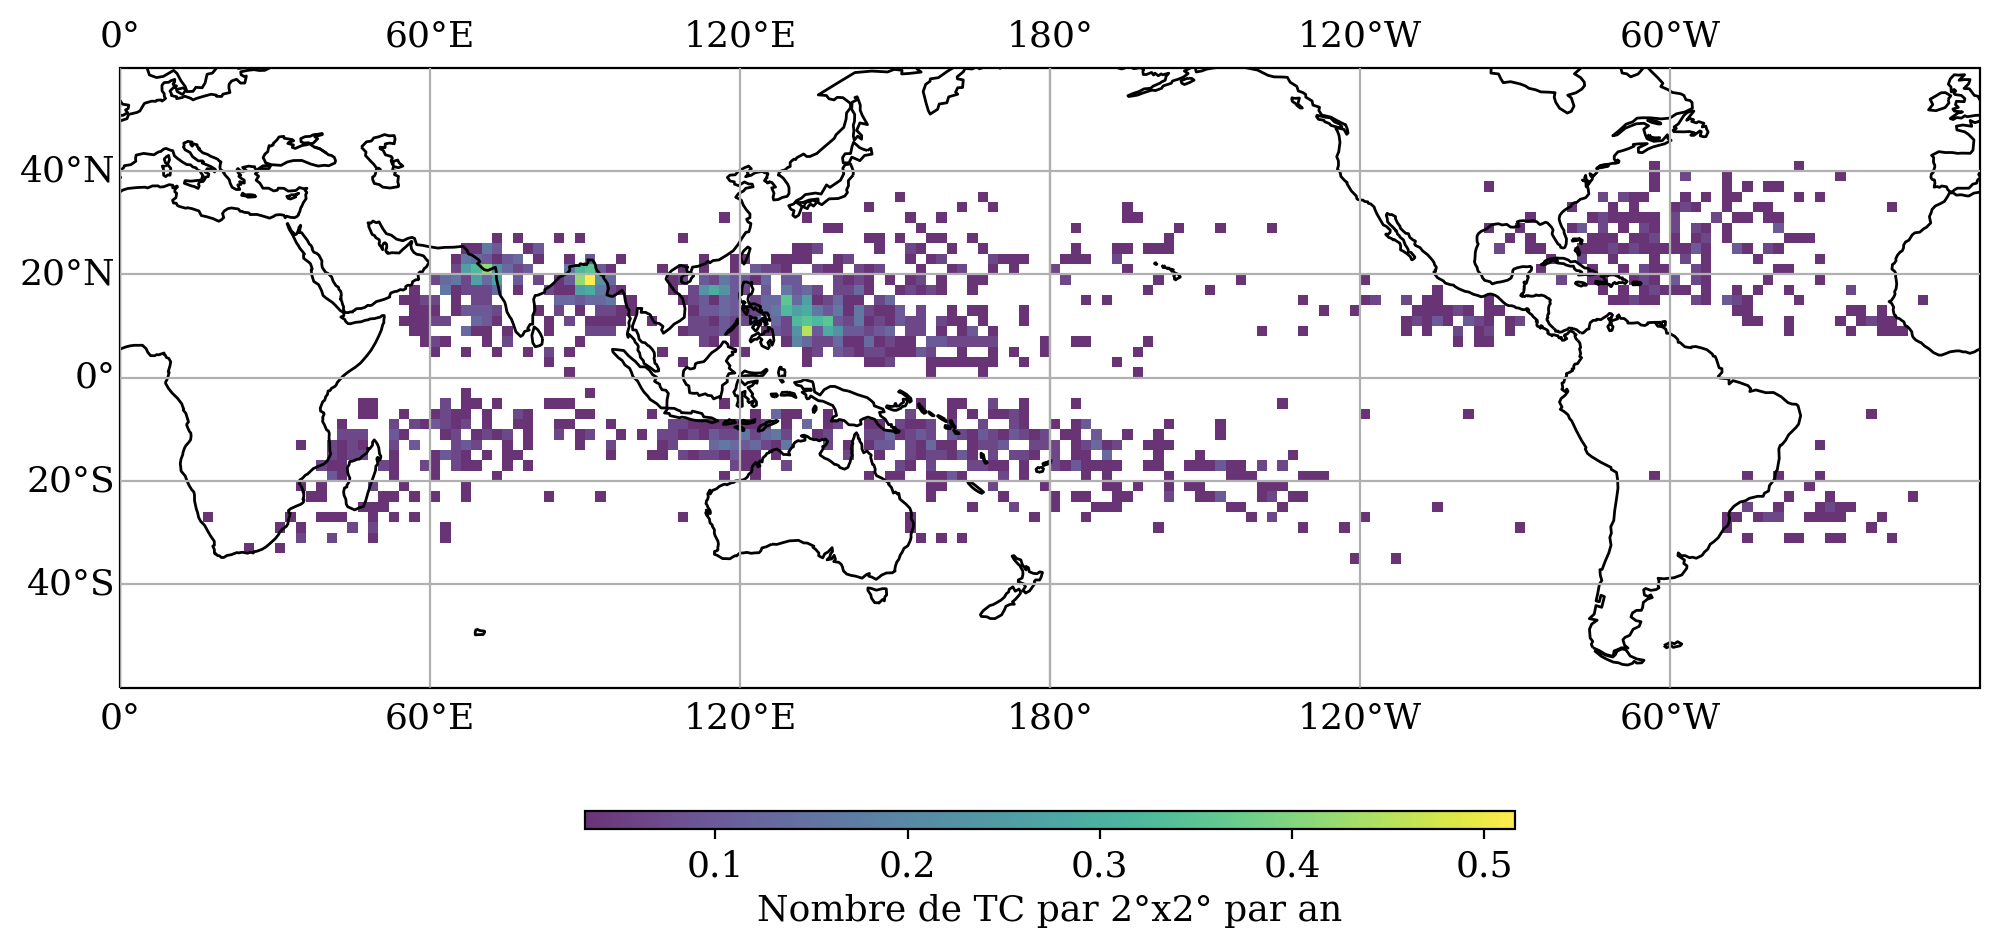
\includegraphics[width=\textwidth]{track_density_PRE625REFT359x.png}
    \caption{Densité annuelle moyenne de cyclogénèses dans la simulation ARPEGE forcée par HadISST1 entre 1980 et 2010, calculée sur une grille régulière de
    \ang{2}$\times$\ang{2}.}
    \label{fig:track_density_PRE625REFT359x}
\end{figure}

La \cref{fig:density_arpege_ibtracs} présente le biais moyen entre la simulation ARPEGE (c.f \cref{fig:track_density_PRE625REFT359x}) et IBTrACS, prise sur la
même période, en termes de densité de probabilité d'occurrence pour pallier à la différence dans la fréquence annuelle des deux jeux de données après
application du filtre du STJ. Dans l'océan Atlantique, la \cref{fig:density_arpege_ibtracs} fait apparaître une légère surestimation dans l'Atlantique sud d'une
part, et une déséquilibre dans l'Atlantique nord avec notamment une sous-évaluation dans le MDR et le GoM, mais une sur-évaluation dans le reste de l'océan. Ce
biais dans l'atlantique nord avec cette simulation est par ailleurs documenté dans \textcite{chauvin_future_2020}. Dans le bassin EPac, l'activité simulée est
fortement sous-estimée. Dans le WPac, un surplus est noté dans ARPEGE en Mer de Chine méridionale et Mer des Philippines, tandis que le reste du bassin voit
sinon un déficit. Dans le bassin NInd, la simulation ARPEGE présente une activité sur-estimée aussi bien en Mer d'Arabie que dans le Golfe du Bengale. Dans
l'hémisphère sud, le biais est plus contrasté. Dans l'océan Indien, on note un biais positif dans le sud-ouest du bassin, autour de Madagascar mais un biais
négatif dans le nord-est, proche de l'équateur. Une répartition du biais similaire mais symétrique est notée dans le bassin Sud Pacifique, avec un biais positif
dans le sud-est et négatif au nord-ouest.

Dans la plupart des bassins, ces motifs de biais sont en fait évocateurs d'une mauvaise localisation des cyclogénèses par le schéma de détection, notamment en
raison de sa tendance connue à détecter les TC un peu tardivement, plutôt que d'un biais avéré dans l'activité simulée. Dans le NAtl, les trajectoires démarrent
le plus souvent de la MDR ou du GoM pour ensuite remonter vers le nord / nord-est. Dans le SInd, les TC se déplacent souvent du nord-est vers le sud-ouest. La
sens de circulation est inversé dans le SPac en raison du flux de mousson en provenance d'ouest qui prend le pas sur la dérive de Coriolis ---~cette dernière
ayant naturellement tendance à déplacer les TC vers l'ouest dans l'hémisphère sud (c.f \cref{sec:conditions_cyclogenese})~--- si bien que les TC s'y déplacent
généralement vers le sud-est. Une détection trop tardive des TC pourrait également expliquer au moins en partie le biais noté dans le WPac (voir aussi
\cref{fig:bassins_TC} du \cref{chap:chapitre_1}, \vpageref{fig:bassins_TC}, pour voir les sens de déplacement des TC dans les bassins océaniques majeurs). Le
\cref{chap:chapitre_2} fait notamment référence à cette tendance que possède le schéma de détection à détecter trop tardivement les TC dans la réanalyse ERA5,
et cet effet est également documenté dans \textcite{bourdin_intercomparison_2022}. Dans ce contexte, les seules régions où il existe un biais réel entre
l'activité simulée par ARPEGE et l'activité observée (outre la différence de fréquence annuelle après passage du filtre) sont le bassin EPac, le NInd, et dans
une mesure bien moindre le Sud Atlantique. L'activité cyclonique telle que simulée dans le modèle ARPEGE et identifiée par le traqueur du CNRM est donc tout
compte fait assez fidèle aux observations. Nous considérons alors que les cyclogénèses issues du schéma de détection du CNRM appliqué à la simulation ARPEGE
peuvent être utilisées comme prédictant pour la construction d'indices de cyclogénèse par régression de Poisson.

\begin{figure}[tb]
    \centering
    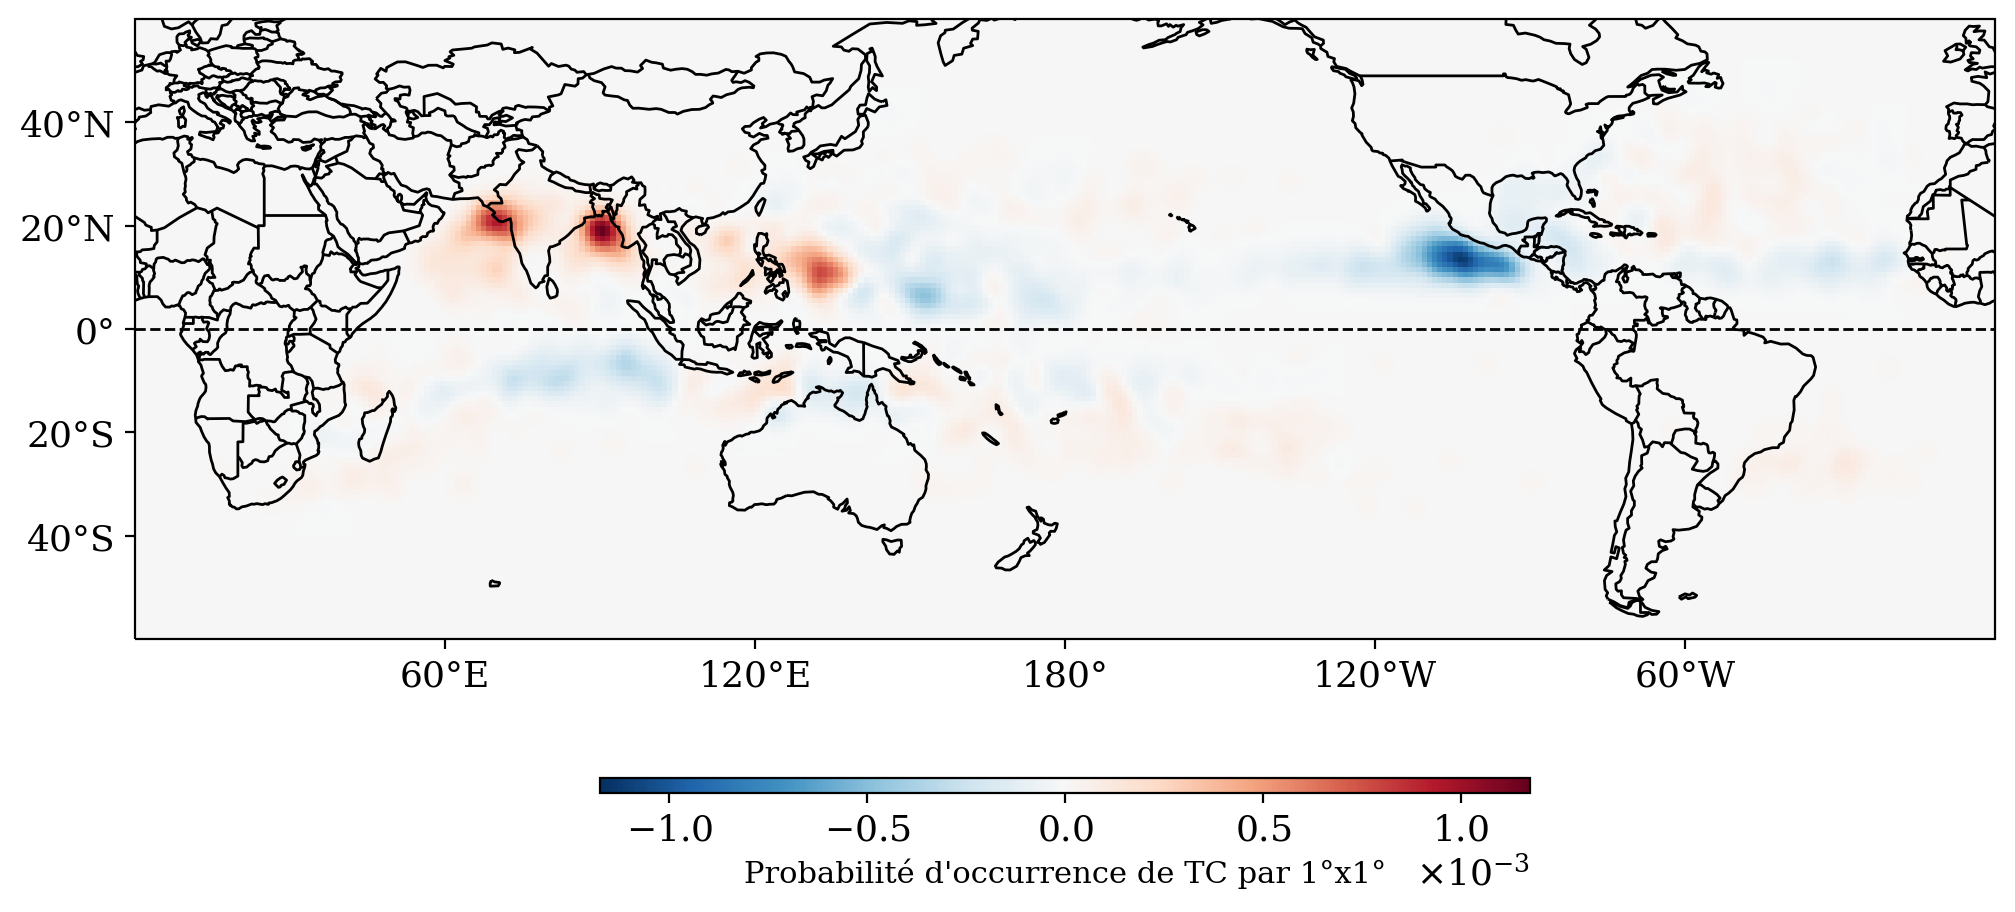
\includegraphics[width=\textwidth]{density_arpege_ibtracs.png}
    \caption{Carte de la différence entre les densités de cyclogénèses moyennes et normalisées ---~lissées au préalable avec un filtre gaussien à \ang{1}
    d'écart-type~--- de la simulation ARPEGE forcée et IBTrACS entre \num{1980} et \num{2010}.}
    \label{fig:density_arpege_ibtracs}
\end{figure}

%La \cref{fig:STJ_PRE625REFT359x} présente quant à elle les moyennes saisonnières de la latitude diagnostiquée par le filtre du STJ pour les deux hémisphères.
%Les variations saisonnières du STJ de la \cref{fig:STJ_PRE625REFT359x} illustrent le caractère dynamique du filtre du STJ, par rapport à une limite en latitude
%fixe. Cette figure met aussi en évidence le caractère saisonnier du filtre, avec un décalage vers les pôles durant les saisons chaudes, et un déport vers
%l'équateur durant la saison froide, les deux étant bien entendu en opposition de phase dans chacun des hémisphères. Cette propriété du seuil dynamique en
%latitude avait déjà été mise en évidence pour le filtre du gradient de géopotentiel à \hPa{200} présenté dans la \cref{sec:filtrage_mid_latitudes}
%(\cref{chap:chapitre_2}), mais n'avait pas été documentée pour le filtre du STJ.

%\begin{figure}[tp]
%    \centering
%    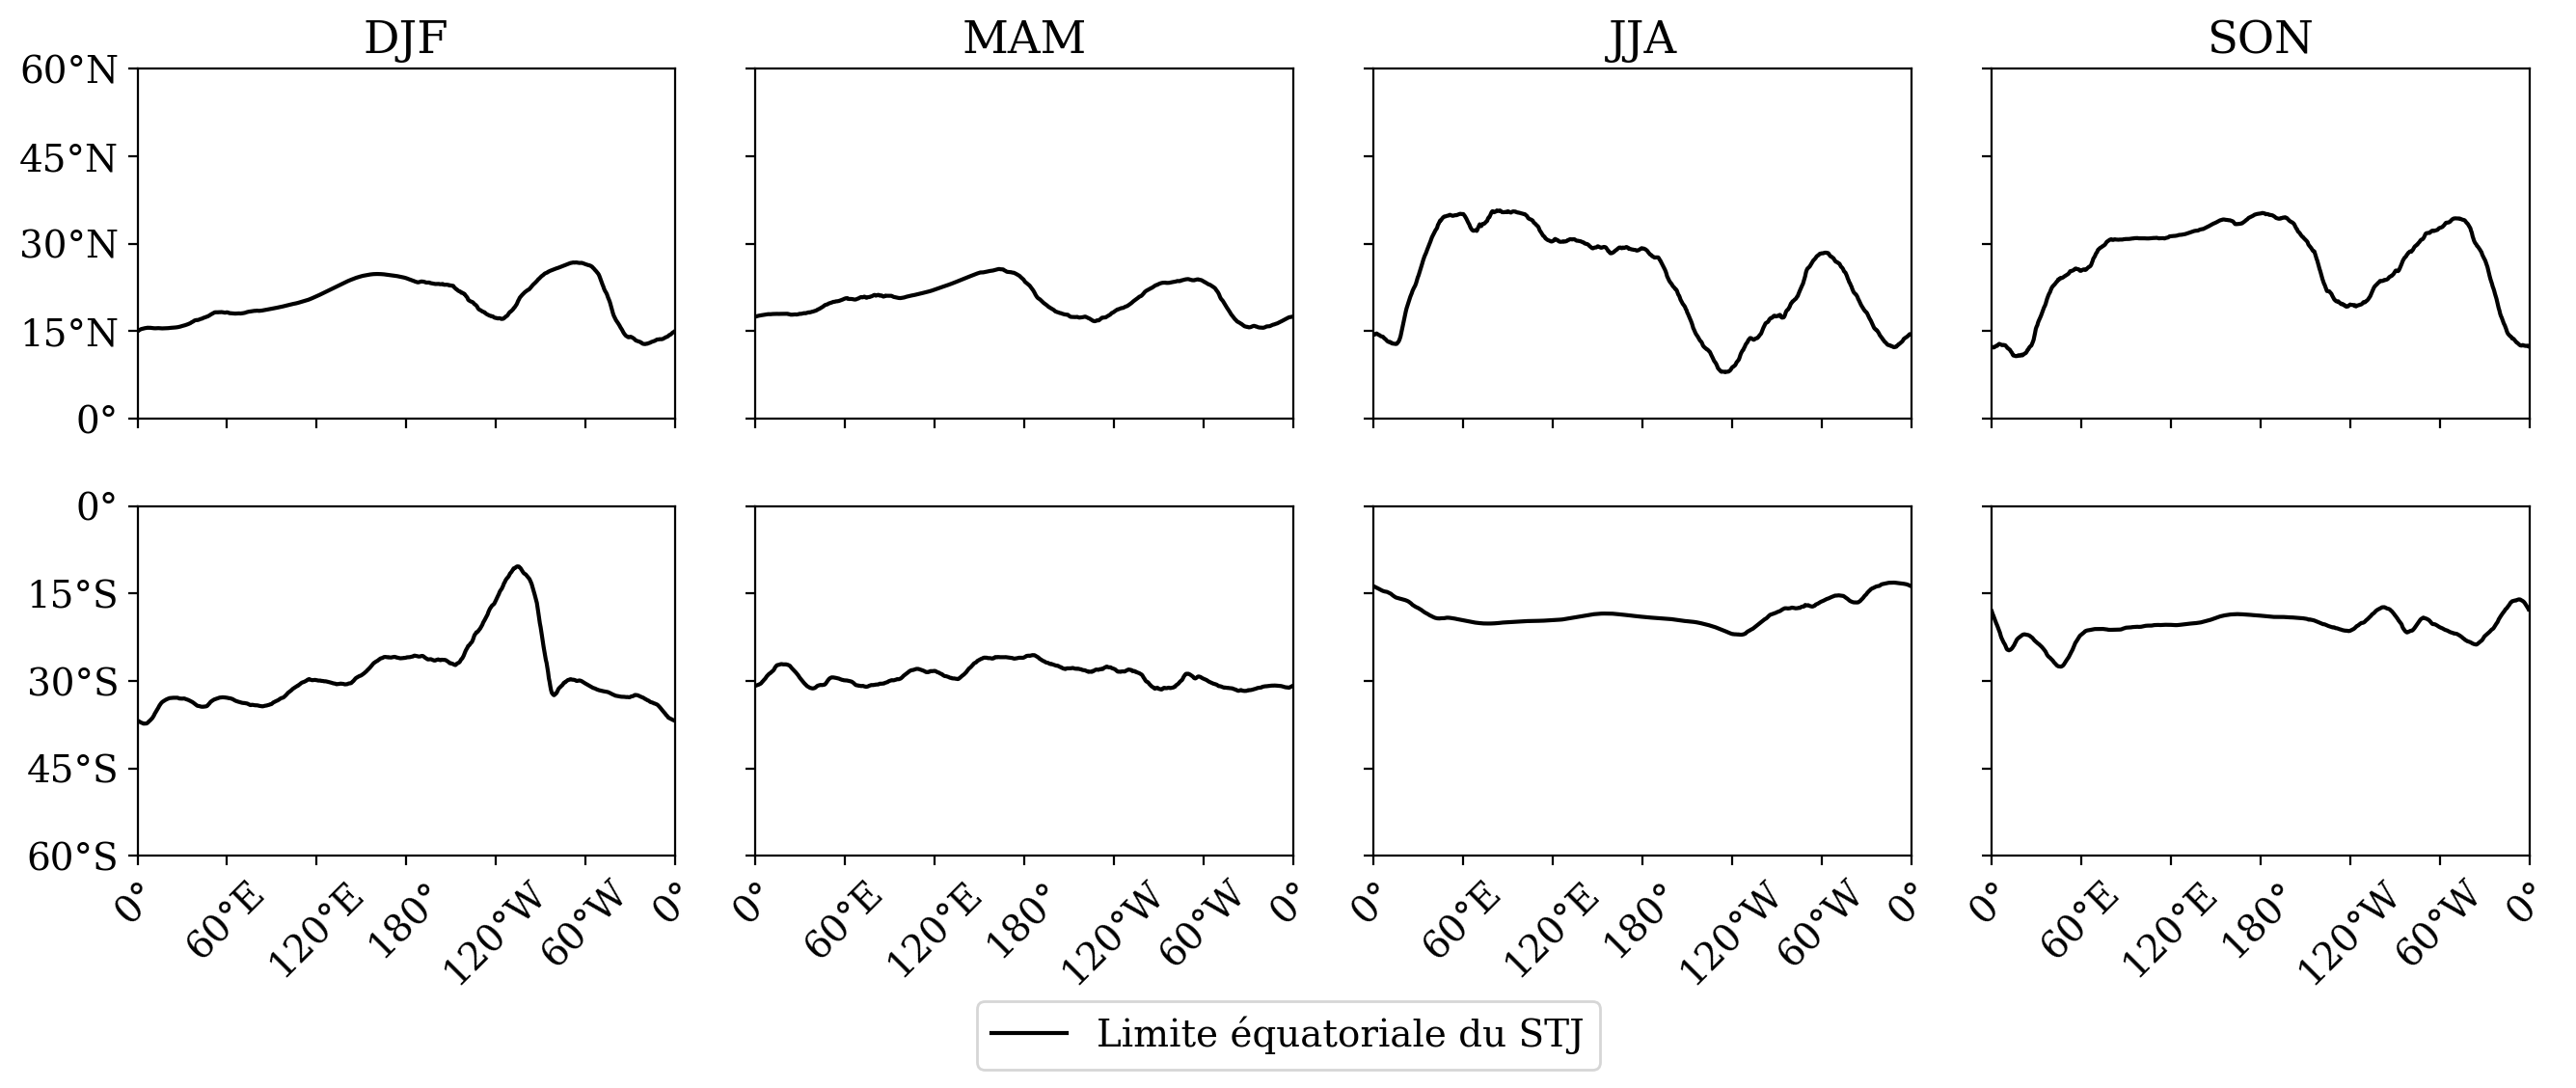
\includegraphics[width=\textwidth]{STJ_season_PRE625REFT359x.png}
%    \caption{Moyennes saisonnières de la latitude de la limite équatoriale du jet subtropical dans la simulation ARPEGE-Climat forcée par HadISST1. Chacune des
%    quatre colonnes correspond à une saison. La première ligne présente le diagnostique pour l'hémisphère nord, tandis que la seconde ligne le présente pour
%    l'hémisphère sud.}
%    \label{fig:STJ_PRE625REFT359x}
%\end{figure}

\subsubsection{Diagnostique ENSO}\label{sec:diag_enso}

Le mode de variabilité El Niño (respectivement El Niña) est caractérisé par une anomalie chaude (respectivement froide) de SST dans l'oćean Pacifique central.
Il existe plusieurs façons de diagnostiquer ce phénomène et qui se distinguent entre elles par la région, ou boîte, utilisée pour calculer l'anomalie de
température, ainsi que par le lissage temporel utilisé. Ces boîtes sont au nombre de \num{4}, réparties entre les côtes de l'Amérique centrale et les îles
Salomon. L'anomalie de SST prise dans une de ces boîtes défini alors un indice El Niño. Ici, nous utilisons l'indice ENSO utilisé pour les besoins
opérationnels de la NOAA, nommé ONI (\textit{Oceanic Niño Index}). L'ONI est défini sur la boîte 3.4, c'est à dire à cheval sur les boîtes \num{3} et \num{4}
(non montrées) et définie entre \ang{120}W et \ang{170}W, et entre \ang{5}S et \ang{5}N. Les anomalies sont lissées sur \num{3} mois glissants, et la référence
climatologique est prise comme la SST moyenne sur la toute la période disponible. La \cref{fig:ONI} présente la boîte 3.4 utilisée pour calculer l'anomalie de
température, ainsi que la série temporelle de l'ONI entre janvier \num{1980} et décembre \num{2010}.

\begin{figure}[htpb]
    \centering
    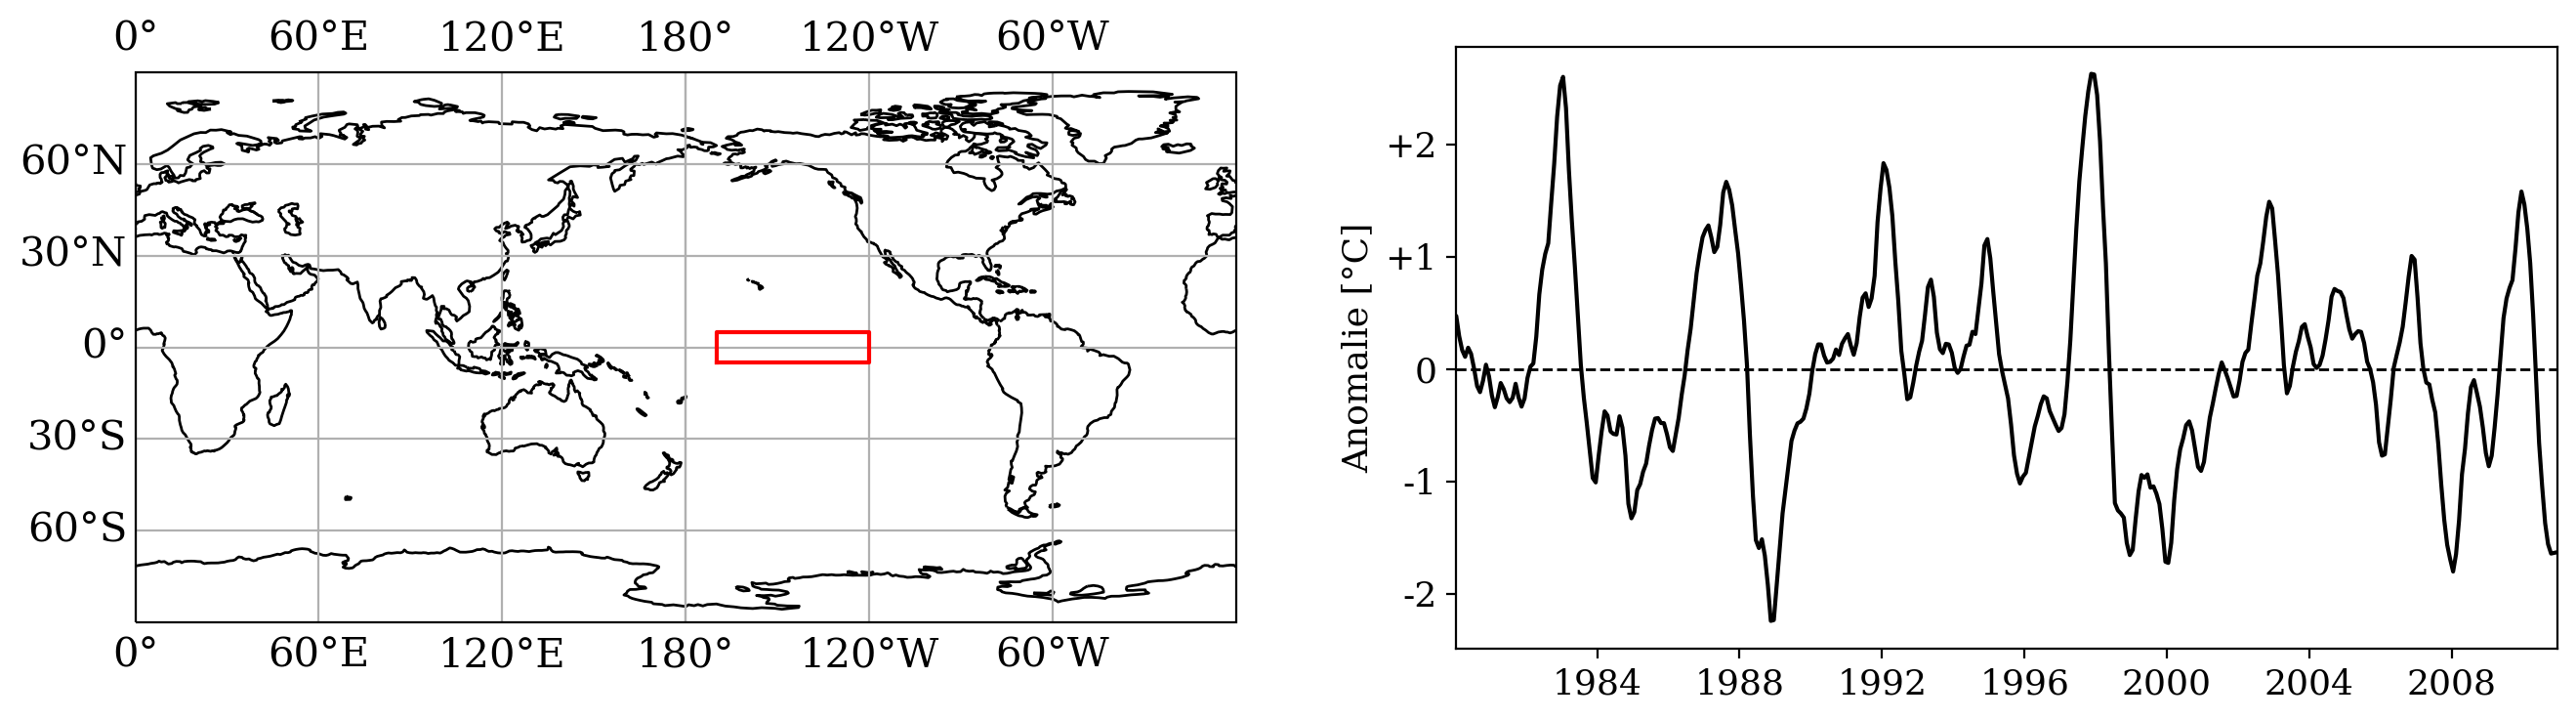
\includegraphics[width=\textwidth]{ONI.png}
    \caption{Boîte 3.4 utilisée pour le calcul de l'ONI (gauche) et série temporelle de l'ONI (droite) évaluée sur la SST mensuelle de la
    simulation ARPEGE forcée par HadISST1.}
    \label{fig:ONI}
\end{figure}

Pour utiliser l'ONI comme prédicteur dans une régression de Poisson, il est nécessaire de le transformer en vecteur de la même taille $m$ (c.f
\cref{chap:chapitre_3}, \cref{sec:regression_poisson}) que les champs spatio-temporels de grande échelle. L'ONI étant, pour un mois donné, un scalaire ; sa
valeur est répliquée en tout point de la grille spatiale souhaitée. Cela revient à considérer que chaque point de l'espace a connaissance à chaque
pas de temps de l'anomalie de SST dans la boîte 3.4.

\subsection{Lien entre ENSO et l'activité cyclonique dans ARPEGE}\label{sec:lien_enso_tracking}

Le lien entre ENSO et l'activité cyclonique tropicale dans les observations et dans les modèles est largement documenté
\parencite{chan_tropical_1985,wu_gcm_1992,landsea_ninosouthern_2000,mcdonald_tropical_2005,lin_enso_2020}. Une phase positive de l'oscillation El-Niño tend à
augmenter la fréquence d'occurence des TC dans certains bassins, notamment dans le Pacifique, et tend à la réduire dans l'océan Indien, et vice versa. Dans
l'Atlantique nord, l'activité cyclonique est traditionnellement anti-corrélée à ENSO, car ce dernier apporte du cisaillement dans l'océan Atlantique. Cependant,
pour déterminer dans quelle mesure l'ajout de l'ONI comme prédicteur dans une régression établie sur les cyclogénèses détectées dans le modèle ARPEGE peut impacter la
fréquence statistiquement modélisée, il convient de quantifier le lien entre l'ONI et l'activité cyclonique dans notre jeu de données.

La \cref{fig:corr_ONI_pt} présente la carte de corrélation entre le nombre annuel de cyclogénèses pour chaque maille d'une grille régulière de \ang{3} de
résolution et l'ONI, aggrégé annuellement de la même façon. Précisons que, à l'instar de toutes les opérations de calcul de variabilité interannuelle
réalisées jusqu'à maintenant, et notamment dans le \cref{chap:chapitre_3}, la fréquence annuelle est calculée pour les saisons cycloniques. Dans l'hémisphère
sud, le nombre de TC pour une saison donnée est donc évalué entre juillet de l'année précédente et juin de l'année courante. Précisons aussi qu'un masque
terre-mer interpolé sur la grille de \ang{3} de résolution est utilisé pour masquer les cyclogénèses détectées sur terre de la
\cref{fig:track_density_PRE625REFT359x}.

\begin{figure}[tpb]
    \centering
    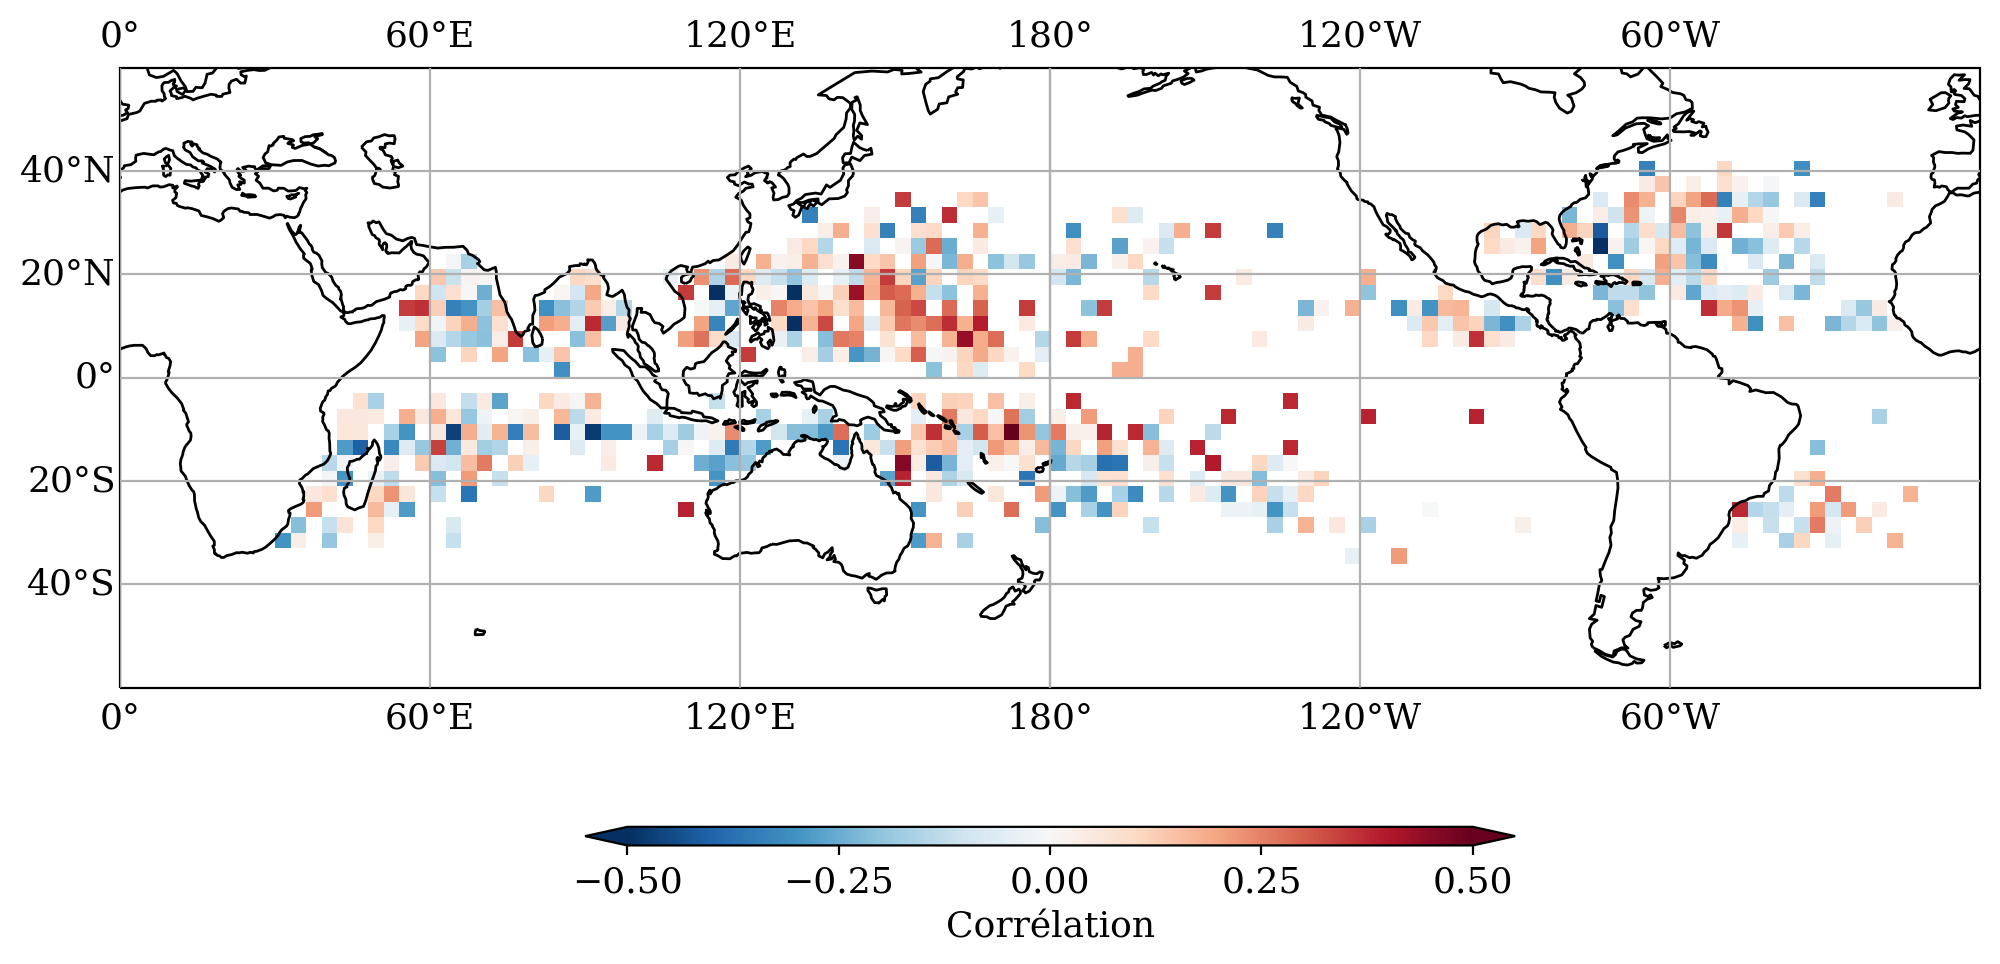
\includegraphics[width=\textwidth]{corr_ONI_tracks.png}
    \caption{Carte de corrélation entre la variabilité interannuelle de l'activité cyclonique par point de grille (\ang{3}x\ang{3}) pour les cyclogénèses
    détectées dans ARPEGE et l'ONI, sur les saisons cycloniques entre \num{1980} et \num{2010}.}
    \label{fig:corr_ONI_pt}
\end{figure}

La \cref{fig:corr_ONI_pt} met en évidence des corrélations contrastées dans les différents bassins d'activité. Le signal le plus clair est noté dans le WPac, à
l'ouest de \ang{180}, avec une corrélation positive dans la plupart des mailles où des cyclogénèses ont été détectées. Certaines dépassent la borne supérieure
de la carte des couleurs fixée à \num{0.5}. Dans le bassin EPac, le peu de cyclogénèses disponibles (voir
\cref{fig:track_density_PRE625REFT359x,fig:density_arpege_ibtracs}) empêche l'interprétation de la corrélation. Dans le SPac, des corrélations positives
relativement fortes sont notées dans la partie nord, tandis que ces dernières s'inversent au delà de \ang{20}S. Dans le bassin SIndE, ENSO apparaît clairement
anti-corrélée à l'activité cyclonique, à l'exception de quelques mailles. Pour les bassins SIndW NInd et NAtl, le signal est plus contrasté mais laisse également
entrevoir dans l'ensemble une possible anti-corrélation.

Pour évaluer le lien entre l'activité cyclonique détectée et la variabilité El Niño dans ces bassins où la \cref{fig:corr_ONI_pt} ne permet pas de dégager une
conclusion nette, la corrélation est évaluée à l'échelle du bassin tout entier. Spécifiquement, les cyclogénèses sont comptabilisées sur la grille d'origine de
la simulation (T359, soit \ang{0.5}), puis l'activité est intégrée spatialement sur les bassins océaniques usuels selon la méthodologie employée dans le
\cref{chap:chapitre_3}. Enfin, la corrélation avec la variabilité interannuelle de l'ONI est évaluée pour chacun des bassins. La
\cref{fig:corr_ONI_bassin} présente les coefficients de corrélation $r$ ainsi que les valeurs-p associées.

\begin{figure}[tpb]
    \centering
    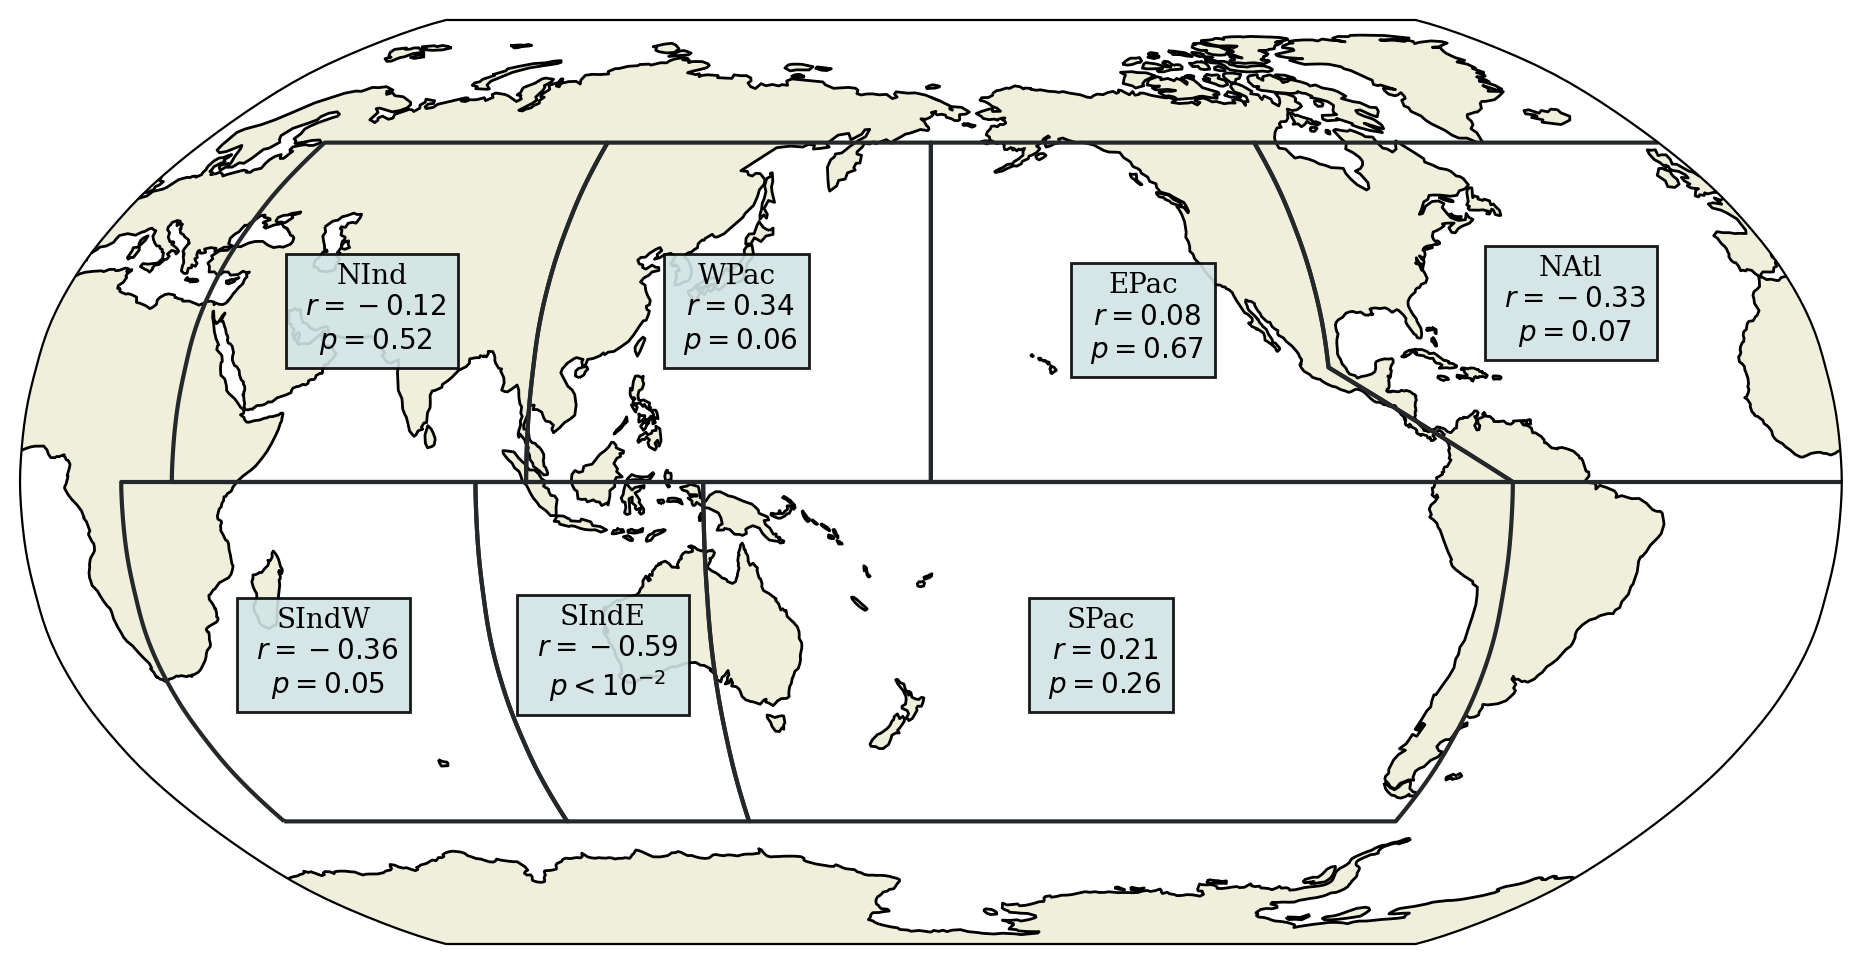
\includegraphics[width=\textwidth]{corr_ONI_bassin}
    \caption{corrélation entre la variabilité interannuelle de l'activité cyclonique détectée dans ARPEGE et l'ONI à l'échelle des bassins océaniques.}
    \label{fig:corr_ONI_bassin}
\end{figure}

Pour les bassins WPac et SIndE, la \cref{fig:corr_ONI_bassin} confirme ce que laisse deviner la \cref{fig:corr_ONI_pt}, à savoir une corrélation dans le
premier, évaluée à \num{0.34} et à la limite de la significativité sous un seuil de \prct{95}, et une anti-corrélation significative dans le second à
\num{-0.59}. La \cref{fig:corr_ONI_bassin} permet également de lever l'ambigüité pour les bassins où le lien est contrasté sur la \cref{fig:corr_ONI_pt}. Ainsi
l'activité cyclonique dans le bassin SIndW est également présenté comme anti-corrélée à l'ONI avec \num{-0.36}, là aussi à la limite de la significativité, et
pareillement dans le bassin NAtl avec \num{-0.33}, bien qu'avec une valeur-p de \num{0.07}. En revanche, le bassin EPac ne présente aucune corrélation, et
celles des bassins NInd et SPac ne sont pas significatives. À titre de référence, cette carte réalisée entre ERA5 et IBTrACS signale une corrélation de
\num{0.54} dans le bassin EPac et de \num{-0.43} dans le bassin NAtl. La corrélation dans le bassin SIndE est inchangée par rapport à celle mesurée ici, mais
les bassins WPac et SIndW sont néanmoins parfaitement décorrélés.

Le lien entre l'activité cyclonique telle que détectée par le schéma de détection du CNRM appliqué au modèle ARPEGE d'une part, et le mode de variabilité El
Niño est dans l'ensemble cohérent. Plusieurs bassins océaniques présentent des corrélations à la limite de la significativité statistique, et c'est par
conséquent dans ces bassins là qu'une éventuelle plus-value de l'ajout de l'ONI comme prédicteur dans une régression de Poisson peut être attendue.

\subsection{Application de la régression}

On applique ici la régression de Poisson selon la même méthodologie employée pour construire l'indice nommé M10 dans la \cref{sec:apport_res_temporel_spatial},
mais appliquée à la simulation ARPEGE. On utilise donc en prédictant les cyclogénèses détectées par le traqueur du CNRM dans la simulation historique ARPEGE
forcée par HadISST1. Ces dernières, de même que les champs de grande échelle utilisés comme prédicteurs, transposées sur une grille régulière de \ang{1} de
résolution et agrégées au pas de temps mensuel. Ici encore, la taille de la matrice $\mathbf{x}$ des prédicteurs est le principal facteur limitant la résolution
spatiale pour réaliser la régression, et est la raison pour laquelle nous n'utilisons pas la grille T359 d'origine. Nous utilisons les mêmes variables
thermiques et dynamiques que pour le TCS et pour les \cref{sec:apport_res_temporel_spatial,sec:indice_regional}, à savoir la vorticité absolue bornée à
\SI{3.7e-5}{\per\second} $\eta$, le cisaillement vertical $V_{\mathrm{shear}}$ entre \hPa{850} et \hPa{200}, l'humidité relative $H$ à \hPa{600} et la SST
relative $T$.

Nous définissons dans un premier temps l'équivalent de l'indice M10 pour ARPEGE, nommé AM10. Nous réalisons ensuite une seconde régression en ajoutant à
ces quatre variables décrivant l'environnement de grande échelle le champ artificiel de l'ONI, défini en tout point de la grille comme l'anomalie
mensuelle de SST dans la boîte 3.4 présentée dans la \cref{sec:diag_enso}. L'indice incluant l'ONI comme prédicteur est nommé OAM10, abrégé en OA. La régression
avec l'ONI comme prédicteur est appliquée aussi bien à l'échelle globale qu'à l'échelle des bassins individuels. Dans le second cas, la méthodologie employée
dans la \cref{sec:indice_regional} pour construire l'indice LM10 est transposée aux prédicteurs et prédictant ARPEGE, notamment pour ce qui concerne la
calibration de l'indice régional sur la fréquence annuelle moyenne inférée par son homologue global. L'indice régional est alors nommé LOAM10, ou simplement
LOA, puisqu'il est entendu que, contrairement au \cref{chap:chapitre_3}, les régressions sont uniquement faites avec les moyennes mensuelles à \ang{1} de
résolution.

Enfin, précisons que les cyclogénèses détectées sur terre sont masquées, si bien que la fréquence annuelle de référence pour la calibration des indices globaux
est réduite à \num{52.32} TC par an. Bien que ce nombre soit bien différent de la fréquence de référence issue IBTrACS utilisée dans le \cref{chap:chapitre_3},
cela n'a aucune importance dès lors que tous les indices sont calibrés sur cette valeur. Le TCS de \textcite{tippett_poisson_2011} est également pris comme
référence pour la comparaison des résultats.

\subsubsection{Régressions globales}

Nous nous intéressons dans un premier temps aux coefficients obtenus pour les régressions globales AM10 et OAM10. L'indice de cyclogénèse AM10 est donné
ci-dessous :
%
\begin{align*}
\tag{AM10}
    \mu &= \exp \big( b_0 + b_\eta \eta + b_{V_{\mathrm{shear}}} V_{\mathrm{shear}} + b_H H + b_T T + \log \cos \phi \big)\\
        &= \exp \big( \num{-18.6861} + \num{2.4363} \eta - \num{0.0192} V_{\mathrm{shear}} + \num{0.0454} H + \num{0.4202} T + \log \cos \phi \big)
\end{align*}
%
Les coefficients de AM10 sont à mettre en regard avec ceux obtenus pour l'indice M10, obtenus entre ERA5 et IBTrACS dans le \cref{chap:chapitre_3}. Ces derniers
peuvent être consultés dans le \cref{tab:fit_spatial_temporel}, \vpageref{tab:fit_spatial_temporel}. Le coefficient $b_H$ est réduit d'environ \num{0.072} à
\num{0.045}, soit une valeur proche du coefficient associé à l'humidité relative du TCS (\num{0.05}). Les coefficients $b_T$ sont quant à eux quasi identiques,
à \num{0.01} près. Cela peut vraisemblablement s'expliquer par le fait que la réanalyse ERA5 assimile des données la SST issue de la base de données HadISST2
jusqu'en \num{2007}. La sensibilité au cisaillement vertical est néanmoins réduite dans AM10, passant d'environ \num{-0.1} dans ERA5 à environ \num{-0.02} dans
ARPEGE, soit une sensibilité cinq fois moindre dans le modèle de climat. Cette valeur du coefficient apparaît néanmoins comme statistiquement significative
(ainsi que tous les autres coefficients) en dépit de sa valeur proche de \num{0}. La régression indique en effet des pourcentiles \prct{2.5} et \prct{97.5} de
respectivement \num{-0.027} et \num{-0.011} pour $b_{V_{\mathrm{shear}}}$, et une valeur-p inférieure à \num{1e-3}. Le coefficient associé à la vorticité
absolue est celui présentant la plus grande différence pasant d'environ \num{1.40} pour M10 à \num{2.44} pour AM10. Une valeur si élévée de $b_\eta$ est
cohérente avec le biais septentrional dans les cyclogénèses détectées dans ARPEGE (voir \cref{fig:density_arpege_ibtracs}), puisqu'il a été largement montré
dans le \cref{chap:chapitre_3} que des valeurs élevées de ce paramètre sont associées à une activité simulée par la régression plus éloignée de l'équateur.

La relation pour l'indice OA est donnée ci-dessous :
%
\begin{align*}
    \tag{OA}
    \mu &= \exp \big( b_0 + b_\eta \eta + b_{V_{\mathrm{shear}}} V_{\mathrm{shear}} + b_H H + b_T T + b_{\mathrm{ONI}} \mathrm{ONI} + \log \cos \phi \big)\\
        &= \begin{aligned}[t]\exp \big( \num{-18.7099} + \num{2.4430}\, \eta - \num{0.0192}\, V_{\mathrm{shear}} \,+\, &\num{0.0454}\, H + \num{0.4221}\, T + \\&\underbrace{\num{0.0638}\, \mathrm{ONI}}_{\mathrm{Indice\ ENSO}} + \log \cos \phi \big)\end{aligned} \end{align*}
%
L'ajout de l'ONI dans la régression ne modifie que très marginalement les coefficients associés aux autres prédicteurs. On ne note qu'une très légère hausse de
$b_\eta$ ainsi qu'une augmentation toute aussi faible de $b_T$. La régression indique cependant une sensibilité positive à l'ONI avec une valeur
$b_{\mathrm{ONI}}$ d'environ \num{0.06}. Cela signifie qu'à l'échelle globale, un changement de $+$\SI{1}{\degreeCelsius} de l'anomalie de SST dans la région
3.4 provoque une hausse de la fréquence d'occurrence modélisée par la régression de l'ordre \prct{6}. Cette valeur apparaît comme statistiquement significative,
avec une valeur-p de \num{0.024}. Il s'agit toutefois de la valeur-p la plus élevée notée jusqu'à maintenant, ces dernières étant sinon systématiquement
inférieures à \num{1e-3}, pour toutes les régressions réalisées dans le \cref{chap:chapitre_3} et dans le chapitre présent. La régression indique un AIC
\parencite[\textit{Akaike Information Criterion},][]{akaike_information_1998} ---~c'est à dire une log-vraisemblance ajustée par le nombre de prédicteurs~---
légèrement réduite par rapport à AM10, passant en effet de \num{24752} à \num{24747}, indiquant une régression de qualité légèrement supérieure lorsque la
variable ONI est introduite.

Néanmoins, la \cref{sec:lien_enso_tracking} montre que le lien entre ENSO et l'activité cyclonique n'est pas uniforme dans l'espace, avec certaines régions
exprimant une corrélation positive, et d'autres une anti-corrélation. Un indice de cyclogénèse formulé sur l'ONI et dont la régression est menée à l'échelle
globale ne peut donc satisfaire le rapport entre ce mode de variabilité et l'activité constatée dans tous les bassins. Sachant cela, il est permis de penser que
le signe positif de $b_{\mathrm{ONI}}$ pour AM10 et sa significativité statistique sont fortement influencés par le bassin WPac, présentant sur la
\cref{fig:corr_ONI_bassin} une corrélation positive, et influençant d'avantage la régression en sa qualité de bassin le plus actif. C'est pour cette raison que la
régression est répétée à l'échelle des bassins.

\subsubsection{Régressions locales}

Le \cref{tab:coefs_LOA} présente les coefficients obtenus pour chacune des régressions faites à l'échelle des bassins océaniques. On s'intéresse tout
particulièrement aux coefficients associés à l'ONI, aux intervalles de confiance ainsi qu'à la significativité de l'ajout de ce prédicteur dans l'indice LOA.

\begin{table}[htpb]
    \centering
    \caption{Coefficients estimés des prédicteurs pour les régressions réalisées à l'échelle des bassins océaniques avec l'ONI. Les pourcentiles \prct{2.5},
    \prct{97.5} des valeurs de $b_{\mathrm{ONI}}$ sont données, de même que la valeur-p pour ce coefficient. La colonne Fréquence indique le nombre de TC par an
    dans chacun des bassins. Chaque indice régional est calibré sur la fréquence annuelle moyenne de l'indice OA pour ce bassin.}
    \label{tab:coefs_LOA}
    \resizebox{\textwidth}{!}{
    \begin{tabular}{lrrrrrrrrrr}
       \toprule\toprule 
       \multicolumn{1}{c}{Bassin} & \multicolumn{6}{c}{Coefficients} & \multicolumn{3}{c}{ONI} & \multicolumn{1}{c}{Fréquence}\\
       \midrule
                                  & $b_0$ & $b_{\eta}$ & $b_{V_{\mathrm{shear}}}$ & $b_H$ & $b_T$ & $b_{\mathrm{ONI}}$ & \prct{2.5} & \prct{97.5} & valeur-p \\
       \midrule
       NAtl    & \num{-16.7188} & \num{2.3260} & \num{-0.0467} & \num{0.0219} & \num{0.3147} & \num{-0.0737} & \num{-0.237} & \num{0.089} & \num{0.376} & \num{6.41} \\
       WPac    & \num{-17.2232} & \num{1.9807} & \num{-0.0321} & \num{0.0501} & \num{0.3457} & \num{0.2184} & \num{0.116} & \num{0.321} & $< 10^{-3}$ & \num{19.40} \\
       EPac    & \num{-16.9821} & \num{2.0161} & \num{-0.0434} & \num{0.0352} & \num{0.3874} & \num{0.0790} & \num{-0.192} & \num{0.350} & \num{0.568} & \num{5.54} \\
       NInd    & \num{-19.9302} & \num{2.8346} & \num{-0.0450} & \num{0.0624} & \num{0.2984} & \num{0.0559} & \num{-0.081} & \num{0.193} & \num{0.425} & \num{3.98} \\
       SPac    & \num{-19.5598} & \num{2.8841} & \num{-0.0397} & \num{0.0340} & \num{0.4375} & \num{0.1797} & \num{0.053} & \num{0.306} & \num{0.005} & \num{10.12} \\ 
       SIndW   & \num{-17.8103} & \num{2.4274} & \num{-0.0367} & \num{0.0385} & \num{0.3672} & \num{-0.1257} & \num{-0.281} & \num{0.030} & \num{0.113} & \num{3.96} \\
       SIndE   & \num{-19.3702} & \num{3.0105} & \num{-0.1024} & \num{0.0403} & \num{0.4964} & \num{-0.1164} & \num{-0.304} & \num{0.071} & \num{0.224} & \num{2.09} \\
       \bottomrule
    \end{tabular}
    }
\end{table}

Les bassins NInd et EPac présentent les valeurs-p associées à leur coefficient $b_{\mathrm{ONI}}$ les plus élevées de toutes, jusqu'à \num{0.568} pour ce
dernier. Ces mêmes bassins présentaient également les liens les moins prononcés entre ENSO et la variabilité interannuelle dans la
\cref{sec:lien_enso_tracking}. Dans le bassin NAtl, la variable ONI apparait non-significative avec une valeur-p de \num{0.376}. Le coefficient
$b_{\mathrm{ONI}}$, valant environ \num{-0.07}, reflète toutefois le signe du coefficient de corrélation de la \cref{fig:corr_ONI_bassin}, et l'intervalle de
confiance ---~bien que traversant le \num{0}~--- est clairement plus situé du côté des valeurs négatives que des valeurs positives, avec des quantiles
\num{0.025} et \num{0.975} de respectivement \num{-0.237} et \num{0.089}. Un constat similaire peut être fait pour les bassins SIndW et SIndE. Les valeurs-p y
sont en effet supérieures à \num{0.05}, mais leurs coefficients, de respectivement \num{-0.13} et \num{-0.12}, de même que leur intervalle de confiance exprimé
par les pourcentiles \prct{2.5} et \prct{97.5}, sont cohérents avec les résultats de la \cref{fig:corr_ONI_bassin}. Notons que des deux bassins, le SIndW
présente la valeur-p la plus faible à \num{0.113}. Enfin, les régressions faites dans les bassins SPac et WPac acceptent toutes deux le prédicteur ONI, avec une
valeur-p $\leq$ \num{0.05}, bien que le premier soit en limite de significativité. Le coefficient $b_{\mathrm{ONI}}$ dans le bassin WPac est par ailleurs le
plus élevé de tous avec \num{0.22}. Cela conforte la suspicion selon laquelle ce bassin influence fortement le signe du coefficient dans l'indice global OA. Il
convient de noter que la significativité dans le bassin SPac d'une part, et la non-significativité dans les bassins SIndW et SIndE n'étaient pas nécessairement
attendues, puisque la \cref{fig:corr_ONI_bassin} fournit l'information inverse. 

Ainsi, les valeurs prises dans les différentes régions par le coefficient $b_{\mathrm{ONI}}$ reflètent, au moins par leur signe, le lien présenté entre la
variabilité El Niño et l'activité cyclonique détectée dans la simulation ARPEGE forcée, en dépit d'une significativité peu franche, à l'exception notable du
bassin WPac. L'alternance entre le signe du coefficient justifie néanmoins la construction d'indices régionaux plutôt que globaux pour l'ajout de prédicteurs
dont l'effet sur l'activité cyclonique n'est pas uniforme dans toutes les régions du monde.

\subsubsection{Variabilité interannuelle}

La \cref{fig:variability_ONI} présente les variations du nombre de TC d'une saison cyclonique à l'autre pour les trois indices établis sur la simulation ARPEGE
historique, pour le TCS ainsi que les variations vues par le schéma de détection du CNRM, pour les sept bassins définis sur la \cref{fig:corr_ONI_bassin}. Le
bassin NInd est en effet inclus dans l'analyse puisque la détection objective de TC dans la simulation permet d'avoir une série complète, contrairement à
IBTrACS dans le \cref{chap:chapitre_3}. Rappelons que, à l'instar de la \cref{sec:indice_regional} du \cref{chap:chapitre_3}, l'indice LOA est en fait défini
par un indice régional différent pour chaque bassin, dont les coefficients sont donnés dans le \cref{tab:coefs_LOA}. La variabilité temporelle du nombre de TC
détectés dans ARPEGE par le traqueur du CNRM est noté \textquote{Tracks}. La significativité statistique de la corrélation entre les séries temporelles des
quatre indices avec les tracks pour chacun des sept bassins est présenté dans le \cref{tab:pvalues_ONI}.

\begin{figure}[p]
    \centering
    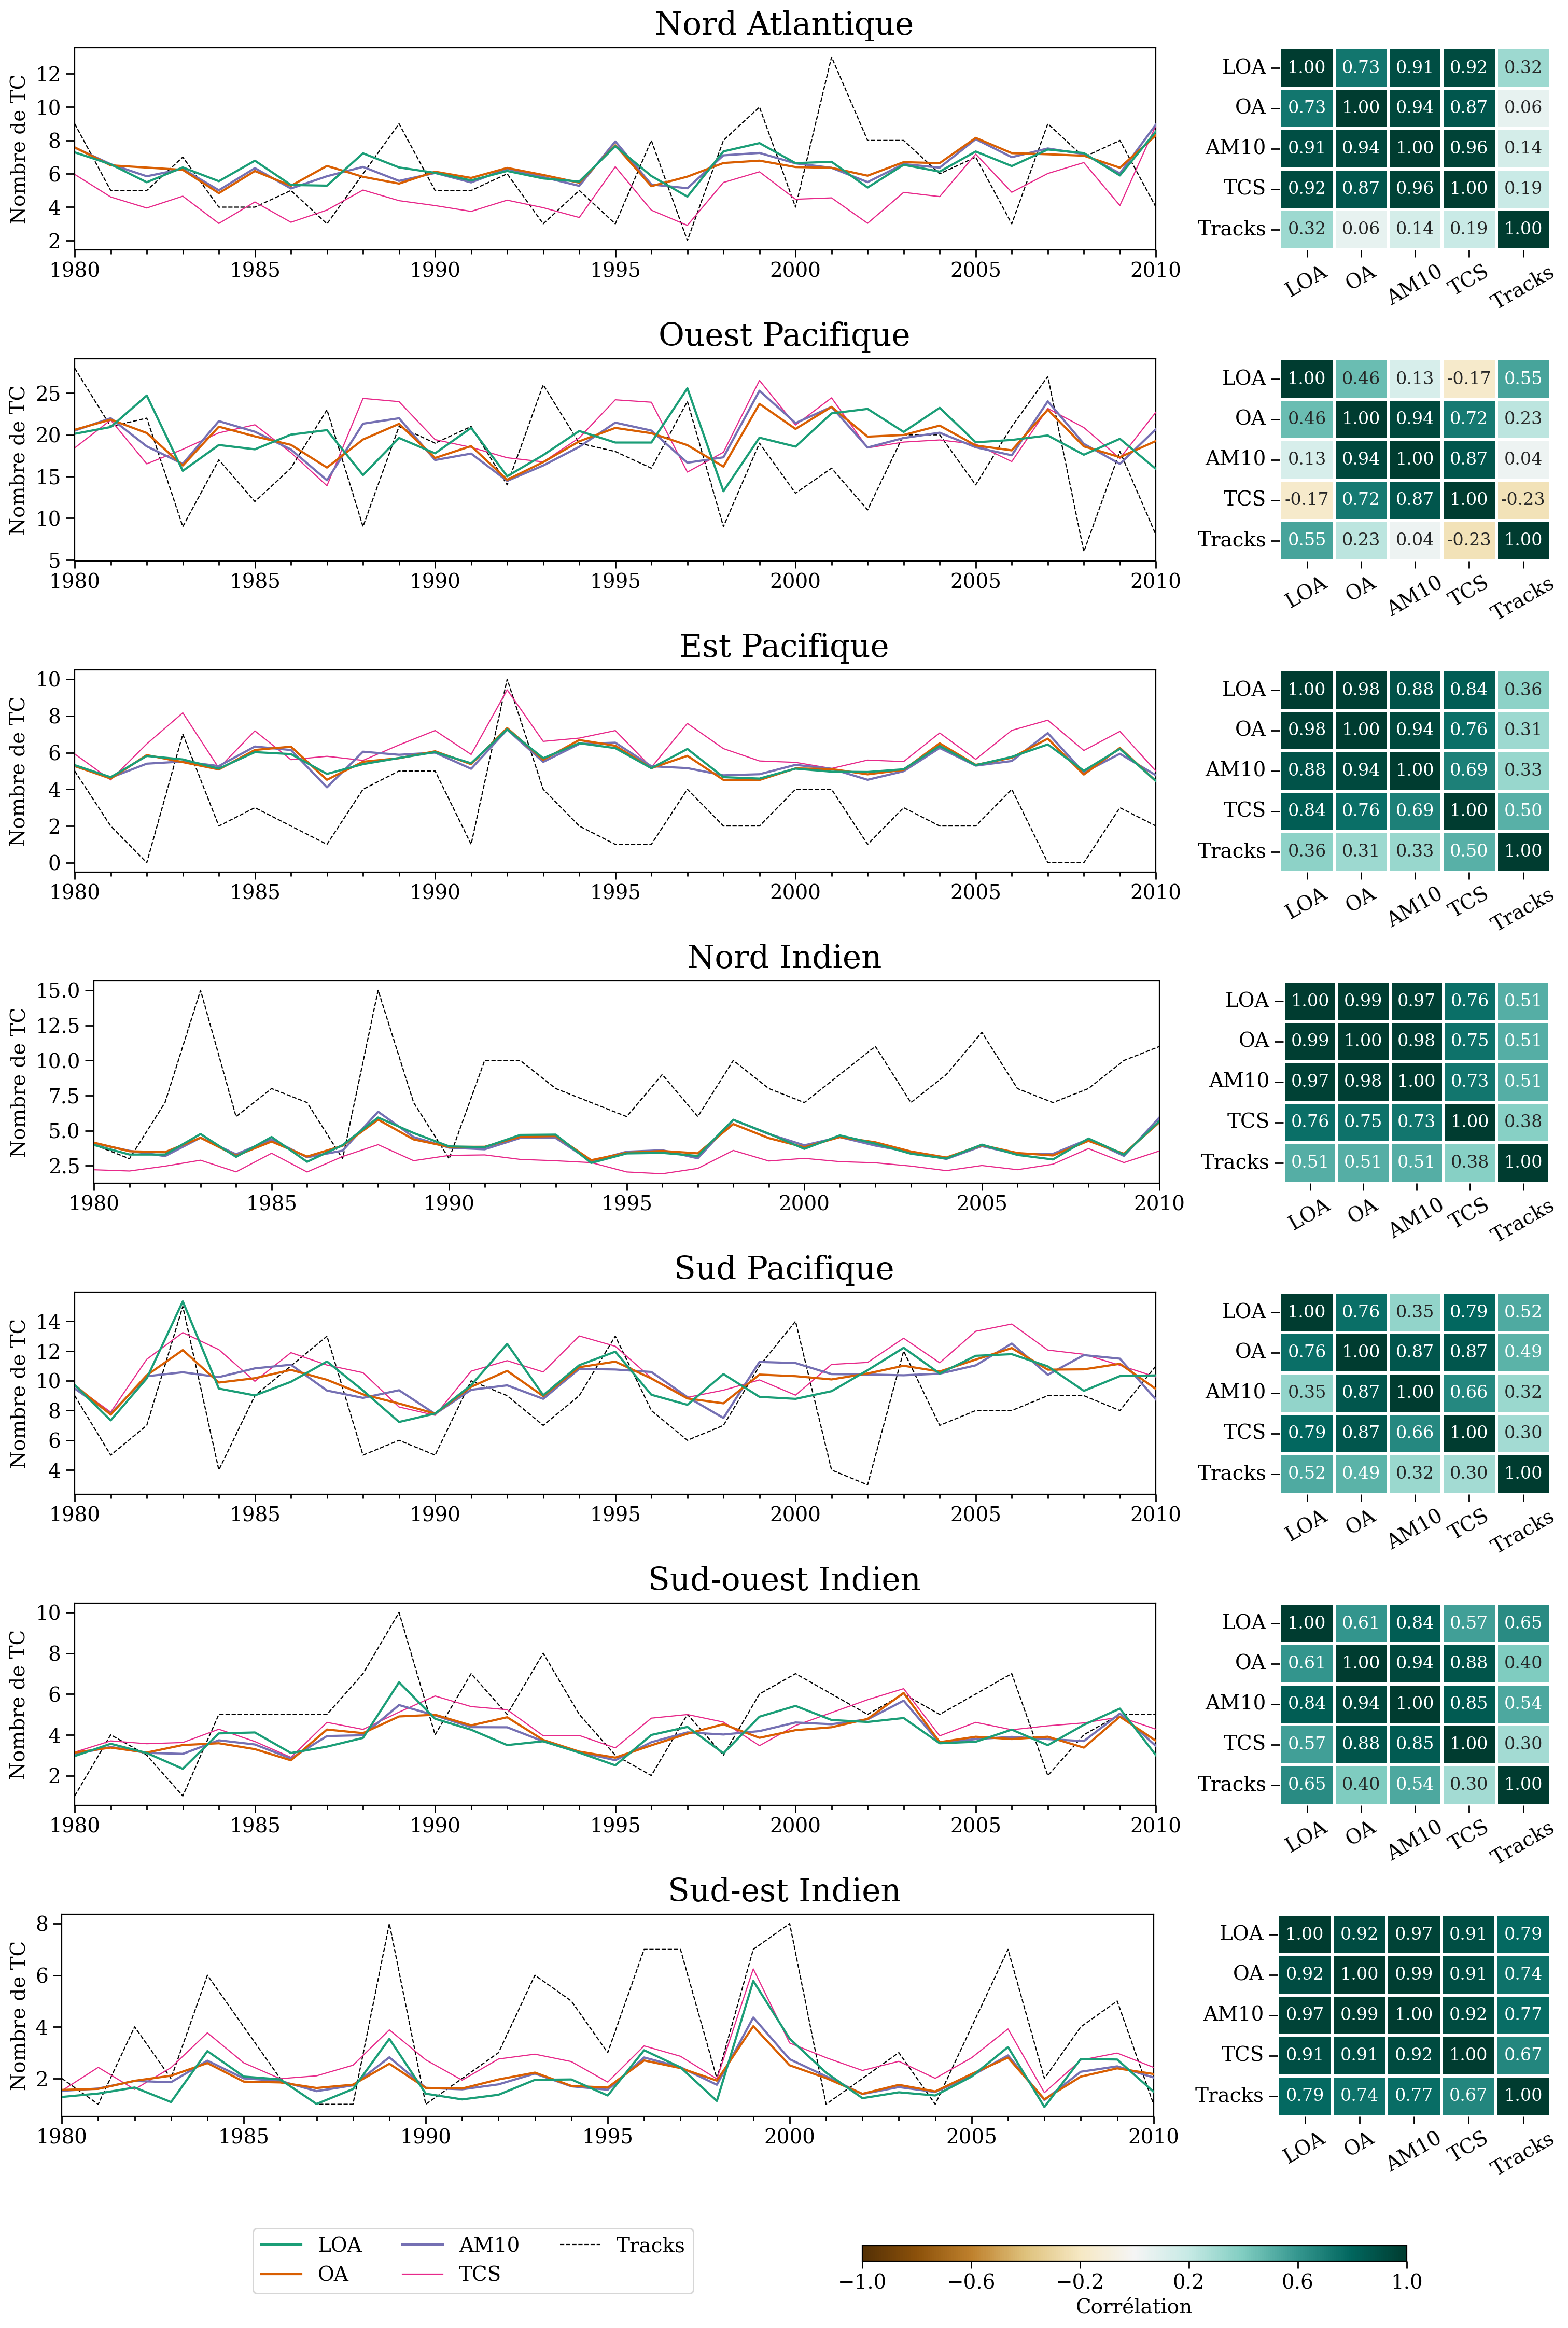
\includegraphics[height=0.94\textheight]{basin_variability_LOA_OA_AM10_TCS_Obs.png}
    \caption{Variabilité interannuelle des trois indices construits sur la simulation ARPEGE, du TCS et issue du schéma de détection (Tracks), ainsi que les
    matrices de corrélation associées.}
    \label{fig:variability_ONI}
\end{figure}

\begin{table}[htpb]
    \centering
    \caption{valeurs-p associées aux corrélations entre la variabilité interannuelle des indices et le tracking (dernière ligne, ou colonne, des matrices de
    corrélation de la \cref{fig:variability_ONI}). Les valeurs renseignées en gras indiquent les valeurs-p en dessous du seuil de \num{0.05}.}
    \label{tab:pvalues_ONI}
    \begin{tabular}{lrrrrrrr}
        \toprule\toprule
        \multicolumn{1}{c}{Indice} & \multicolumn{7}{c}{Bassin géographique}\\
        \midrule
                                   & NAtl & WPac & EPac & NInd & SPac & SIndW & SIndE \\
        \midrule
        LOA  & \num{0.084} & \textbf{\num{0.001}} & \textbf{\num{0.045}} & \textbf{\num{0.003}} & \textbf{\num{0.002}} & $\mathbf{< 10^{-3}}$ & $\mathbf{< 10^{-3}}$ \\
        OA   & \num{0.747} & \num{0.213} & \num{0.086} & \textbf{\num{0.003}} & \textbf{\num{0.005}} & \textbf{\num{0.026}} & $\mathbf{< 10^{-3}}$ \\
        AM10 & \num{0.438} & \num{0.839} & \num{0.069} & \textbf{\num{0.003}} & \num{0.077} & \textbf{\num{0.002}} & $\mathbf{< 10^{-3}}$ \\
        TCS  & \num{0.307} & \num{0.214} & \textbf{\num{0.004}} & \textbf{\num{0.036}} & \num{0.097} & \num{0.097} & $\mathbf{< 10^{-3}}$ \\
        \bottomrule
    \end{tabular}
\end{table}

La \cref{fig:variability_ONI} montre que l'ajout de l'indice ENSO comme prédicteur dans la régression parvient, avec un effet variable selon les bassins, à
modifier la variabilité interannuelle inférée par les indices de cyclogénèse d'une part, et à améliorer la corrélation entre cette variabilité et celle mesurée
par le schéma de détection de cyclones tropicaux dans la simulation ARPEGE d'autre part. Notons que le nombre annuel de TC simulé par l'indice LOA est significativement
corrélé à l'activité détectée par le traqueur dans tous les bassins géographiques à l'exception du Nord Atlantique. Dans ce dernier, le LOA présente néanmoins
une amélioration sensible de la corrélation associée à une valeur-p en limite de significativité par rapport aux autres indices.

L'impact le plus marquant se trouve dans le bassin Ouest Pacifique. La corrélation ---~quasi-nulle pour AM10, et négative pour TCS~--- passe de \num{0.23} pour
OA à \num{0.53} pour LOA. La corrélation entre le LOA et les tracks est hautement significative avec une valeur-p de \num{0.001}. Rappelons que le prédicteur
ONI présente également la significativité la plus élevée dans la régression de Poisson pour ce bassin (\cref{tab:coefs_LOA}) et aussi le coefficient
$b_{\mathrm{ONI}}$ le plus élevé. Les performances intermédiaires de l'indice OA proviennent alors sans doute de la sensibilité diminuée de l'indice à ce
prédicteur dans la régression globale. La valeur du coefficient $b_{\mathrm{ONI}}$ est en effet le coefficient présentant le plus grand changement entre
l'indice global OA et l'indice régional LOA, avec une sensibilité à la variable ONI \num{3.4} supérieure dans l'indice LOA par rapport à l'indice OA.

Les bassins SPac et SIndW voient également une amélioration sensible de leur variabilité interannuelle lorsque le prédicteur ONI est introduit dans la
régression régionale. Notons que dans ces deux bassins, la corrélation est significative pour OA et LOA, mais que la corrélation est diminuée pour OA par
rapport à AM10 dans le SIndW. L'indice LOA dépasse en revanche la corrélation de l'indice AM10. Dans le SPac, la corrélation temporelle de l'indice OA est
intermédiaire entre AM10 et LOA. Cela provient du fait que la variabilité ENSO est anti-corrélée dans le Sud Indien, et corrélée dans le Sud Pacifique, tandis
que le signe de $b_{\mathrm{ONI}}$ dans l'indice OA imprime un lien positif entre El Niño et l'activité cyclonique. Ainsi, bien que OA soit significativement
corrélé aux tracks dans le SIndW, la significativité est sensiblement plus marquée pour LOA dans ce bassin, avec une valeur-p inférieure à \num{1e-3}, et un
coefficient de corrélation parmi les plus élevés de tous les bassins de \num{0.65}, malgré un défaut d'amplitude.

Dans le SIndE et NInd, tous les indices sont significativement corrélés aux tracks. Dans le NInd, la corrélation est invariante entre AM10, OA et LOA, et les
séries temporelles indiscernables. Tous trois présentent néanmoins une amélioration par rapport au TCS. Notons que les valeurs du coefficient $b_{\mathrm{ONI}}$
entre OA et LOA sont proches l'une de l'autre, et particulièrement basses. Il n'est donc pas surprenant de ne voir aucun impact de l'ajout de la variable ONI
par rapport à AM10. Cette région fait partie de celles ---~avec le bassin EPac~--- pour lesquelles les cyclogénèses détectées par le traqueur dans ARPEGE
présentent un biais positif (négatif pour le bassin EPac) prononcé par rapport à IBTrACS (voir \cref{fig:density_arpege_ibtracs}). Ce biais est d'ailleurs
apparent sur la \cref{fig:variability_ONI} puisque tous les indices sous-estiment largement l'activité issue du traqueur dans la région. Dans le SIndE, on note
le même phénomène que dans le SIndW ; à savoir une amélioration entre AM10 et TCS, une dégradation entre OA et AM10 et de nouveau une amélioration pour LOA par
rapport aux trois autres. Cet effet s'explique de la même manière que pour le SIndW, mais il convient de noter que les différences dans les performances des
trois indices sont nettement moins prononcées que dans le bassin SIndW.

Le bassin EPac se démarque quelque peu des autres bassins puisque le TCS se place en première position, et dont la significativité est la plus franche avec une
valeur-p de \num{0.004}. Outre le TCS, seul l'indice LOA atteint également la significativité avec une valeur-p de \num{0.045}, mais un coefficient de
corrélation moindre par rapport à ce dernier. Comme mentionné précédemment, l'activité cyclonique détectée dans le modèle ARPEGE dans ce bassin présente un
important biais négatif. Il est alors possible que ce biais soit lié aux mauvaises performances des indices construits à partir des cyclogénèses détectées.

Enfin, notons que l'amplitude de la variabilité interannuelle simulée par les indices de cyclogénèse dans la plupart des bassins est sous-estimée. L'amplitude
dans le bassin WPac est la plus ressemblante à l'activité détectée, suivie du bassin SPac, notamment pour l'indice LOA. Une explication possible à cela pourrait
trouver son origine dans la nature même de la régression de Poisson. Rappelons en effet que les coefficients de la régression expriment des sensibilités de la
fréquence d'occurrence attendue des TC aux changements dans les prédicteurs. En particulier, ces sensibilités expriment une modification relative de la
fréquence modélisée par la régression. Ainsi, les deux régions les plus actives que sont les bassins WPac et SPac, dans lesquels les indices AM10, OA et LOA
produisent respectivement \num{19.4} TC par an et \num{10.12} TC par an\footnote{La fréquence d'occurrence moyenne simulée par le TCS n'est pas toujours alignée
sur celle des trois autres indices, selon les régions. Ce dernier est néanmoins également calibré pour produire \num{52.32} TC par an à l'échelle
globale.}\footnote{Rien n'impose que la fréquence d'occurrence moyenne de l'indice AM10 dans chacun des bassins soit égale à celle des indices OA et LOA. La
proximité entre les coefficients des deux indices ainsi que la faible sensibilité au prédicteur ONI dans l'indice OA laissent toutefois penser que les
fréquences moyennes régionales sont très proches, ce qui est également corroboré par la \cref{fig:variability_ONI}.} (\cref{tab:coefs_LOA}) présentent également
la plus grande amplitude. Inversement, les bassins où l'activité inférée par les indices est faible tendent à présenter une faible amplitude.

\subsection{Discussion}

Cette section s'est concentrée sur l'introduction d'un diagnostique du mode de variabilité El Niño dans la construction d'un indice de cyclogénèse par
régression de Poisson. Pour cela une simulation réalisée avec le modèle ARPEGE-Climat sur la période \num{1979}~--~\num{2010}, forcée par le jeu de données
HadISST1 est utilisée pour fournir les prédicteurs de grande échelle. Le schéma de détection du CNRM est utilisé pour comptabiliser les cyclogénèses dans la
simulation, lesquelles étant préalablement filtrées par le diagnostique du jet subtropical présenté dans le \cref{chap:chapitre_2}. La répartition spatiale de
l'activité cyclonique détectée dans la simulation ARPEGE est jugée suffisamment réaliste pour utiliser ces données comme prédictant dans une régression de
Poisson, malgré un biais négatif important dans le bassin Est Pacifique, et un biais au contraire positif dans le bassin Nord Indien (voir
\cref{sec:tracking_arpege}). L'utilisation du diagnostique ENSO dans la construction d'indices de cyclogénèse consiste à apporter artificiellement, et de la
manière la plus explicite possible, l'information concernant la phase du mode de variabilité océanique dans la régression, de façon à ce que chaque point de
grille ait accès à cette information à chaque pas de temps.

Trois indices sont construits sur les champs mensuels de la simulation interpolés sur une grille régulière de \ang{1} de résolution horizontale : Un indice
global basé sur les prédicteurs du TCS (AM10), un indice global similaire auquel est ajouté la variable ONI (OA) et un indice régional ---~c'est à dire dont les
coefficients sont fonction du bassin océanique~--- possédant lui aussi la variable ONI comme prédicteur (LOA). La régionalisation de l'indice avec l'ONI est en
effet jusitifée par le fait que l'effet du phénomène El Niño sur la modulation de l'activité cyclonique est positif dans certaines régions, et négatif dans
d'autres (voir \cref{sec:lien_enso_tracking}). Les résultats montrent que l'ajout de la variable ONI comme prédicteur dans la construction de l'indice parvient
efficacement à améliorer la représentation de la variabilité interannuelle inférée par l'indice de cyclogénèse régional, avec l'impact le plus frappant
concernant le bassin Ouest Pacifique. Seules les deux régions dans lesquelles l'activité cyclonique simulée par ARPEGE présente un biais important ne montrent
pas d'amélioration notable suite à l'introduction de ce nouveau prédicteur. Cette amélioration de la variabilité interannuelle se fait cependant au détriment du
sens physique que porte sinon l'indice de cyclogénèse, la philosophie originelle consistant en effet à n'utiliser que des variables intervenant (supposément)
directement dans le processus physique de cyclogénèse.

L'amélioration de la variabilité interannuelle lorsque la phase du mode de variabilité El Niño est explicitement renseignée interroge également sur la manière
dont un indice de cyclogénèse perçoit les télé-connexions. En effet, l'activité cyclonique simulée par le modèle atmosphérique ressent l'effet de l'ENSO, comme
en atteste la \cref{sec:lien_enso_tracking} (et notamment les \cref{fig:corr_ONI_pt,fig:corr_ONI_bassin}). \textcite{camargo_use_2007} montrent par ailleurs que
le GPI de \textcite{emanuel_tropical_2004} reproduit fidèlement les anomalies spatiales de l'activité cyclonique liées à l'ENSO, et mettent en évidence
l'importance du rôle joué par chacun des prédicteurs, notamment de l'humidité relative en moyenne troposphère et le cisaillement vertical du vent. Ces
variables, ainsi que la SST (absente du GPI), faisant partie intégrante des indices utilisés ici, une bonne réponse dans la variabilité interannuelle de ces
derniers à la phase de l'ENSO pouvait être attendue. De surcroît, la variabilité interannuelle des indices utilisés ici n'incluant pas la variable ONI, à savoir
l'AM10 et le TCS, réagissent tout de même à la phase de l'ENSO, mais dans une mesure amoindrie et de manière moins consistante. On peut en effet le voir pendant
l'épisode de 1983 dans le bassin SPac, mais aussi en 1992 et 1997 dans le bassin EPac et ainsi qu'en 1999 dans le bassin SIndE, pour ne citer que quelques
exemples. La capacité des indices de cyclogénèse à réagir à ce mode de variabilité est en outre documentée depuis les travaux de
\textcite{watterson_seasonal_1995} (c.f \cref{sec:intro_indices} du \cref{chap:chapitre_1}).

Sachant cela, l'introduction de la variable ONI aurait pu être tout à fait redondante et n'apporter aucune plus-value dans la régression. C'est d'ailleurs une
interprétation possible aux significativités pour le moins hésitantes associées à ce prédicteur dans le \cref{tab:coefs_LOA}. En effet, le champ spatial
artificiel de l'ONI, construit en répliquant la valeur (scalaire) du diagnostique en tout point de l'espace, ne contient par définition aucune variabilité
spatiale. Or, les résultats obtenus dans le \cref{chap:chapitre_3} montrent que la régression de Poisson vise avant toute autre chose à fournir la meilleure
vraisemblance spatiale entre les prédicteurs et le prédictant. Malgré cela, l'utilisation de l'ONI comme prédicteur et d'un coefficient $b_{\mathrm{ONI}}$
associé, quand bien même ce dernier n'est pas statistiquement significatif, améliore sensiblement la corrélation entre la variabilité interannuelle de l'indice
avec la variabilité détectée dans la plupart des bassins. Chercher à améliorer la représentation de la variabilité interannuelle inférée par un indice de
cyclogénèse par l'ajout de nouveaux prédicteurs apparaît donc possible, mais la méthodologie de construction d'un indice par régression de Poisson ne semble pas
être le mode opératoire le mieux adapté à cette tâche.

% Rappelons également que la significativité associée à la variable ONI dans l'indice régional ne reflète pas nécessairement celle entre la série temporelle de
% l'ONI et la variabilité temporelle de l'activité détectée dans la simulation (c.f \cref{fig:corr_ONI_bassin}), avec notamment un lien clair entre ENSO et les
% cyclogénèses détectées dans les bassins SIndW et SIndE, mais moins évident dans le SPac, tandis que l'ajout du prédicteur dans ces régions pour la construction
% de l'indice LOA renvoie le message inverse. Une explication à ce qui peut alors

\section{Tendances introduites par le déficit de saturation d'humidité}

Le déficit de saturation d'humidité atmosphérique, comme déjà évoqué dans le \cref{chap:chapitre_1} (\cref{sec:projections_futures}), constitue une variable
d'intérêt pour l'étude de l'activité cyclonique tropicale dans le contexte de réchauffement climatique. Dans une atmosphère plus chaude, celui-ci augmente du
fait de la dépendance de la pression de vapeur saturante à la température, tandis que l'humidité relative est projetée comme approximativement constante. Le
déficit de saturation d'humidité, que l'on appelera par la suite VPD (\textit{Vapour-Pressure Deficit}), et noté $s$, est défini ici comme la différence $s =
e_s - e$, où $e_s$ est la pression de vapeur saturante et $e$ la pression partielle de la vapeur d'eau : $e / e_s$. Le VPD se distingue donc de l'humidité
relative définie par le ratio entre la pression partielle de la vapeur d'eau et la pression de vapeur saturante. \textcite{emanuel_hurricanes_2008} montrent via
une expérience de descente d'échelle statistique que des simulations climatiques dans lesquelles le déficit de saturation est maintenu constant présentent une
augmentation du nombre de TC, alors qu'elles indiquent sinon une baisse lorsque ce paramètre n'est pas influencé. Ces résultats ont conduit à la formulation
modifiée du GPI proposée par \textcite{emanuel_tropical_2010} ---~mentionnée dans la \cref{sec:relations_empiriques} du \cref{chap:chapitre_3}~--- dans laquelle
l'humidité relative est remplacée par une mesure adimensionnelle du déficit de saturation d'entropie humide, similaire au VPD. Cet indice appliqué aux
simulations CMIP5 présente cependant toujours un signal divergeant (c'est à dire une augmentation de l'activité) en climat plus chaud.
\textcite{camargo_testing_2014} montrent à l'inverse que certaines combinaisons de prédicteurs dans un indice de cyclogénèse construit par régression de Poisson
peuvent aboutir à une fréquence d'occurrence à la baisse en climat futur, notamment lorsque le VPD est introduit.

On s'intéresse dans cette nouvelle et dernière section à l'apport du VPD en lieu et place de l'humidité relative à \hPa{600} dans un indice de cyclogénèse
construit par une régression de Poisson. En particulier, puisqu'il a été mis en évidence que la variabilité interannuelle d'un tel indice était difficile à
améliorer, nous nous intéressons plutôt à la recherche et à l'analyse de tendances dans la variabilité du nombre de TC d'une année sur l'autre.

\subsection{Déficit de saturation d'humidité}

Conformément à \textcite{camargo_testing_2014}, le VPD est intégré verticalement en chaque point de grille. L'intégration verticale bénéficie en effet de
l'avantage, par rapport à une moyenne, de ne pas être influencé par les valeurs très faibles dans les dernières couches de l'atmosphère. Le déficit de
saturation d'humidité s'exprime traditionnellement en \SI{}{\kilo\pascal}, et l'intégrale sur plus d'une vingtaine de niveaux verticaux d'espacement variable
amène à de larges valeurs numériques. Pour cette raison, le VPD intégré sur la colonne est exprimé ici en $10^6$~\SI{}{\pascal\squared}. Cela se traduit par une
plage de valeurs comprise entre \SI{1e6}{\pascal\squared} et \SI{62e6}{\pascal\squared}, soit un ordre de grandeur comparable aux autres prédicteurs, et en
particulier à l'humidité relative ---~que le VPD remplace~--- et donc \textit{in fine} à une valeur du coefficient $b_s$ qu'il est possible de comparer à $b_H$.
En effet, puisque les coefficients expriment des sensibilités pour des changements unitaires, l'application d'un facteur d'échelle au prédicteur se répércute de
la même manière sur son coefficent dans la régression. En outre, et bien que \textcite{camargo_testing_2014} ne précisent pas l'unité utilisée pour le déficit
de saturation intégré sur la colonne, notre valeur de $b_s$ est du même ordre de grandeur que celle proposée pas ces derniers.

La régression est faite selon l'exact même mode opératoire que pour l'indice AM10 construit dans la section précédente, et l'indice M10 établit sur ERA5 avant
lui (voir \cref{sec:apport_res_temporel_spatial}). La relation ainsi établie est donnée ci-dessous :
%
\begin{align*}
%\tag{VPD}
    \mu &= \exp \big( b_0 + b_\eta \eta + b_{V_{\mathrm{shear}}} V_{\mathrm{shear}} + b_{s} \, s + b_T T + \log \cos \phi \big)\\
        &= \exp \big( \num{-13.5399} + \num{2.3765} \, \eta - \num{0.0179} \, V_{\mathrm{shear}} \underbrace{- \num{0.1238} \, s}_{\mathrm{VPD}} + \num{0.6204} \, T + \log \cos \phi \big)
\end{align*}
%
Le coefficient $b_s$ est donné à \mypm{-0.1238}{0.007}, avec des pourcentiles \prct{2.5} et \prct{97.5} de respectivement \num{-0.138} et \num{-0.110}. Le
prédicteur est donc hautement significatif dans la régression. À titre de référence, le coefficient trouvé dans \textcite{camargo_testing_2014}, entre la
réanalyse NCEP et IBTrACS, est de $+$\num{0.13}. La différence du signe s'explique par le fait qu'ici, et contrairement à \textcite{camargo_testing_2014}, le
VPD est défini positif, si bien qu'une grande valeur de $s$ est associée à une colonne atmosphérique particulièrement sèche, et donc défavorable à la
cyclogénèse. Notons que la régression faite sur ERA5 et IBTrACS (protocole M10) avec l'intégrale verticale du VPD en remplacement de l'humidité relative conduit
à une valeur similaire avec $b_s^{\mathrm{ERA5}} \sim \num{-0.17}$. Avec les moyennes climatologiques (protocole C10), on a $b_s^{\mathrm{ERA5}} \sim
\num{-0.14}$, ce qui se rapproche encore d'avantage du coefficient de \textcite{camargo_testing_2014}, lesquels utilisent également des moyennes
climatologiques. Ici, les coefficients $b_\eta$ et $b_{V_{\mathrm{shear}}}$ demeurent quasiment inchangés par rapport à AM10. La seule différence notable se
trouve dans la sensibilité à la SST relative, qui passe d'environ \num{0.42} à \num{0.62} ici. Une augmentation du même ordre de grandeur est notée sur ERA5
(M10 comme C10), avec par exemple un passage de $b_T^{\mathrm{ERA5}}$ de \num{0.41} à \num{0.62} pour M10. \textcite{camargo_testing_2014} présentent le même
constat avec un coefficient de SST relative passant de \num{0.35} à \num{0.57} lorsque le VPD est introduit. L'effet du VPD sur les coefficients de la
régression entre la fréquence d'occurrence des TC et l'environnement de grande échelle apparaît donc robuste entre NCEP, ERA5 et les observations IBTrACS d'un
côté, et notre simulation ARPEGE forcée par HadISST1 et les cyclogénèses issues du schéma de détection de cyclones tropicaux de l'autre.

La \cref{fig:diff_VPD_AM10} présente la différence entre les moyennes temporelles de l'indice construit avec le VPD sur ARPEGE et l'indice AM10. L'effet du VPD
dans la répartition spatiale de l'activité simulée par l'indice est variable selon les bassins (voir aussi le \cref{tab:tendances_PRE625REFT359x} pour la façon
dont la fréquence annuelle est affectée par ce nouveau prédicteur dans chacun des bassins). Le VPD amène notamment à deux changements intéressants, présentés
dans les grossissements sur la \cref{fig:diff_VPD_AM10}. Ces deux régions correspondent à des domaines où ni IBTrACS, ni les cyclogénèses détectées dans ARPEGE
ne recensent d'activité (voir \cref{fig:acgi_ibt,fig:track_density_PRE625REFT359x}). Par conséquent, toute activité simulée par un indice de cyclogénèse
construit sur ces données constitue nécessairement un biais de l'indice\footnote{Les indices de cyclogénèse présentés dans ce manuscrit ne sont par définition
    jamais strictement nuls, ce qui est d'autant plus vrai pour les régressions de Poisson définis comme une fonction exponentielle. Dans les régions évoquées,
    il ne fait toutefois aucun doute que le niveau d'activité des indices dépasse celui d'un simple bruit de fond.}. Or, un tel biais est présent dans le GPI et
    le TCS (de même que tous les indices dérivés du TCS définis dans ce manuscrit jusqu'à maintenant, et notamment AM10), lequel est brièvement mentionné dans
    le \cref{chap:chapitre_3} (\cref{sec:proprietes_indices}).

\begin{figure}[tb]
    \centering
    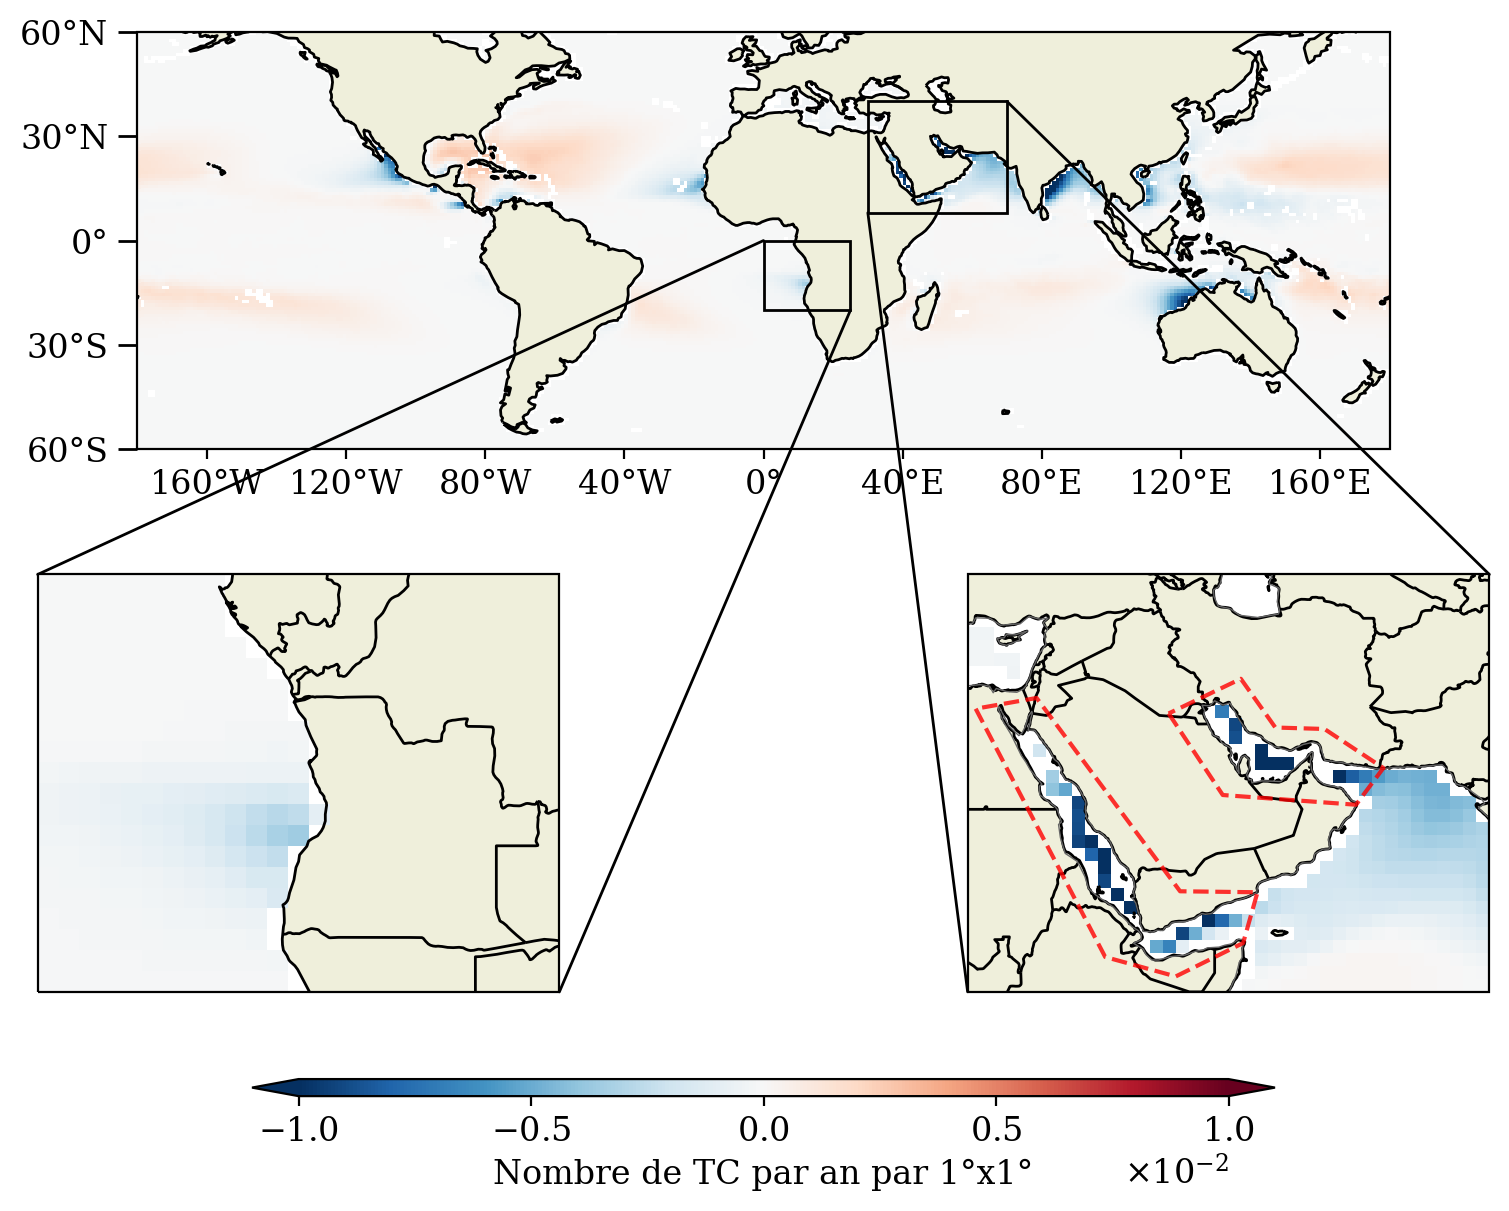
\includegraphics[width=\textwidth]{carte_diff_VPD_AM10.png}
    \caption{Carte des différences annuelles moyennes entre l'indice utilisant avec VPD et AM10. Les deux grossissements montrent la côte au large de l'Angola
    (entre \ang{0}E et \ang{25}E, et \ang{20}S et l'équateur) d'une part et la région du Golfe Persique et de la Mer Rouge (entre \ang{30}E et \ang{70}E, et
    \ang{8.5}N et \ang{40}N) d'autre part.}
    \label{fig:diff_VPD_AM10}
\end{figure}

Le premier changement, et le plus conséquent des deux, consiste en la réduction du biais positif dans le Golfe Persique ainsi qu'en Mer Rouge, deux sous-régions
du bassin NInd. En Mer Rouge (incluant le Golfe d'Aden, entre le Yémen et la Somalie, délimitée en pointillés sur la \cref{fig:diff_VPD_AM10}), la fréquence
annuelle moyenne entre \num{1980} et \num{2010} inférée par l'indice AM10 est de \num{0.2} TC par an, tandis qu'elle est réduite à \num{0.02} TC par an pour
l'indice incluant le VPD. Réciproquement, dans le Golfe Persique (en incluant également le Golfe d'Oman à l'embouchure, voir délimitations en pointillés), la
fréquence est réduite de \num{0.1} TC par an à \num{0.005} TC par an pour l'indice incluant le VPD par rapport à AM10. Le CYGP quant à lui ne présente pas ce
problème (rappelons qu'il ne dépend pas de l'humidité relative). Il en résulte que la production de TC dans ces régions est purement une conséquence de
l'utilisation de l'humidité relative dans la formulation des indices. Le deuxième domaine dont la représentation de l'activité est amélioré par l'introduction
du VPD est au large des côtes de l'Angola. L'indice incluant le VPD voit sa fréquence réduite de \num{0.14} TC par an (AM10, le TCS y simule quant à lui
\num{0.17} TC par an) à \num{0.04} TC par an. Cette région ne présente pas d'activité cyclonique dans les observations, ni dans les données du traqueur, mais
tous les indices dépendant de l'humidité relative y présentent un bias positif, si bien que toute réduction de l'activité représente une amélioration.

Le \cref{tab:tendances_PRE625REFT359x} présente l'analyse des tendances dans le nombre annuel de TC dans la simulation ARPEGE forcée par HadISST1, tels que vus
par plusieurs indices et par le schéma de détection. L'indice défini ici, dans lequel le VPD remplace l'humidité relative y est sobrement appelé VPD. Sont
également inclus dans ce tableau : l'indice AM10 ; l'indice M10 du \cref{chap:chapitre_3}, évalué sur la simulation ARPEGE historique de la même manière que les
autres ---~et notamment re-calibré pour fournir \num{52.32} TC par an à l'échelle globale entre \num{1980} et \num{2010}~--- et dont les coefficients furent
obtenus en appliquant la régression entre ERA5 et IBTrACS entre \num{1980} et \num{2019} ; le TCS et enfin les données issues du schéma de détection. La
comparaison avec M10 en plus du TCS se justifie par le fait que l'indice M10 peut être vu comme une version actualisée du TCS.

\begin{table}[htpb]
    \centering
    \caption{Tendances dans le VPD, AM10, M10, TCS ainsi que les cyclogénèses détectées dans la simulation ARPEGE forcée par HadISST1, sur les saisons 1980 à
    2010. La pente est donnée en TC par décennie. La pente en \% est en TC par année rapportée à la fréquence annuelle moyenne de l'indice dans ce bassin.
    La fréquence annuelle moyenne est donnée dans la dernière colonne. Les lignes en gras indiquent une tendance significative à
    \prct{95}}
    \label{tab:tendances_PRE625REFT359x}
    \begin{adjustbox}{height=0.425\textheight}
    \begin{tabular}{llrrrr}
    \toprule
     &  & Pente & Pente (\%) & valeur-p & Fréquence \\
    \midrule
    \multirow[t]{5}{*}{Nord Atlantique} & VPD & 0,214 & 0,301 & 0,276 & 7.1 \\
     & AM10 & \textbf{0,446} & \textbf{0,697} & \textbf{0,018} & \textbf{6.4} \\
     & M10 & \textbf{0,602} & \textbf{1,273} & \textbf{0,011} & \textbf{4.7} \\
     & TCS & \textbf{0,645} & \textbf{1,365} & \textbf{0,014} & \textbf{4.7} \\
     & Tracks & 0,585 & 0,959 & 0,252 & 6.1 \\
    \midrule
    \multirow[t]{5}{*}{Ouest Pacifique} & VPD & -0,121 & -0,062 & 0,845 & 19.3 \\
     & AM10 & 0,268 & 0,138 & 0,622 & 19.4 \\
     & M10 & 0,407 & 0,194 & 0,527 & 21.0 \\
     & TCS & 0,467 & 0,234 & 0,458 & 19.9 \\
     & Tracks & -1,347 & -0,777 & 0,251 & 17.3 \\
    \midrule
    \multirow[t]{5}{*}{Est Pacifique} & VPD & -0,191 & -0,350 & 0,297 & 5.5 \\
     & AM10 & -0,023 & -0,041 & 0,882 & 5.5 \\
     & M10 & 0,079 & 0,126 & 0,712 & 6.3 \\
     & TCS & 0,018 & 0,029 & 0,934 & 6.3 \\
     & Tracks & -0,565 & -1,989 & 0,195 & 2.8 \\
    \midrule
    \multirow[t]{5}{*}{Nord Indien} & VPD & -0,069 & -0,252 & 0,646 & 2.7 \\
     & AM10 & 0,031 & 0,078 & 0,862 & 4.0 \\
     & M10 & 0,048 & 0,164 & 0,753 & 2.9 \\
     & TCS & 0,071 & 0,257 & 0,529 & 2.8 \\
     & Tracks & 0,911 & 1,125 & 0,126 & 8.1 \\
    \midrule
    \multirow[t]{5}{*}{Sud Pacifique} & VPD & 0,315 & 0,289 & 0,293 & 10.9 \\
     & AM10 & \textbf{0,494} & \textbf{0,491} & \textbf{0,039} & \textbf{10.1} \\
     & M10 & 0,579 & 0,554 & 0,063 & 10.5 \\
     & TCS & 0,478 & 0,439 & 0,138 & 10.9 \\
     & Tracks & 0,121 & 0,143 & 0,847 & 8.5 \\
    \midrule
    \multirow[t]{5}{*}{Sud-ouest Indien} & VPD & 0,138 & 0,323 & 0,359 & 4.3 \\
     & AM10 & 0,274 & 0,694 & 0,061 & 3.9 \\
     & M10 & \textbf{0,382} & \textbf{0,907} & \textbf{0,049} & \textbf{4.2} \\
     & TCS & \textbf{0,341} & \textbf{0,770} & \textbf{0,034} & \textbf{4.4} \\
     & Tracks & 0,391 & 0,798 & 0,336 & 4.9 \\
    \midrule
    \multirow[t]{5}{*}{Sud-est Indien} & VPD & 0,061 & 0,400 & 0,613 & 1.5 \\
     & AM10 & 0,114 & 0,555 & 0,380 & 2.1 \\
     & M10 & 0,175 & 0,805 & 0,351 & 2.2 \\
     & TCS & 0,175 & 0,650 & 0,351 & 2.7 \\
     & Tracks & 0,323 & 0,893 & 0,506 & 3.6 \\
    \midrule
    \multirow[t]{5}{*}{Global} & VPD & 0,332 & 0,063 & 0,743 & 52.3 \\
     & AM10 & \textbf{1,633} & \textbf{0,312} & \textbf{0,045} & \textbf{52.3} \\
     & M10 & \textbf{2,297} & \textbf{0,439} & \textbf{0,009} & \textbf{52.3} \\
     & TCS & \textbf{2,232} & \textbf{0,427} & \textbf{0,007} & \textbf{52.3} \\
     & Tracks & 0,129 & 0,025 & 0,932 & 52.3 \\
    \bottomrule
    \end{tabular}
\end{adjustbox}
\end{table}

Test

%--------------------------------------
\section{Synthèse}

\end{document}
